\section{Sơ đồ trình tự và Sơ đồ hoạt động}

\subsection{Xử lý ra/vào cho các thành viên của trường}
\subsubsection{Sơ đồ hoạt động (Activity Diagram)}
\begin{figure}[H]
    \centering
    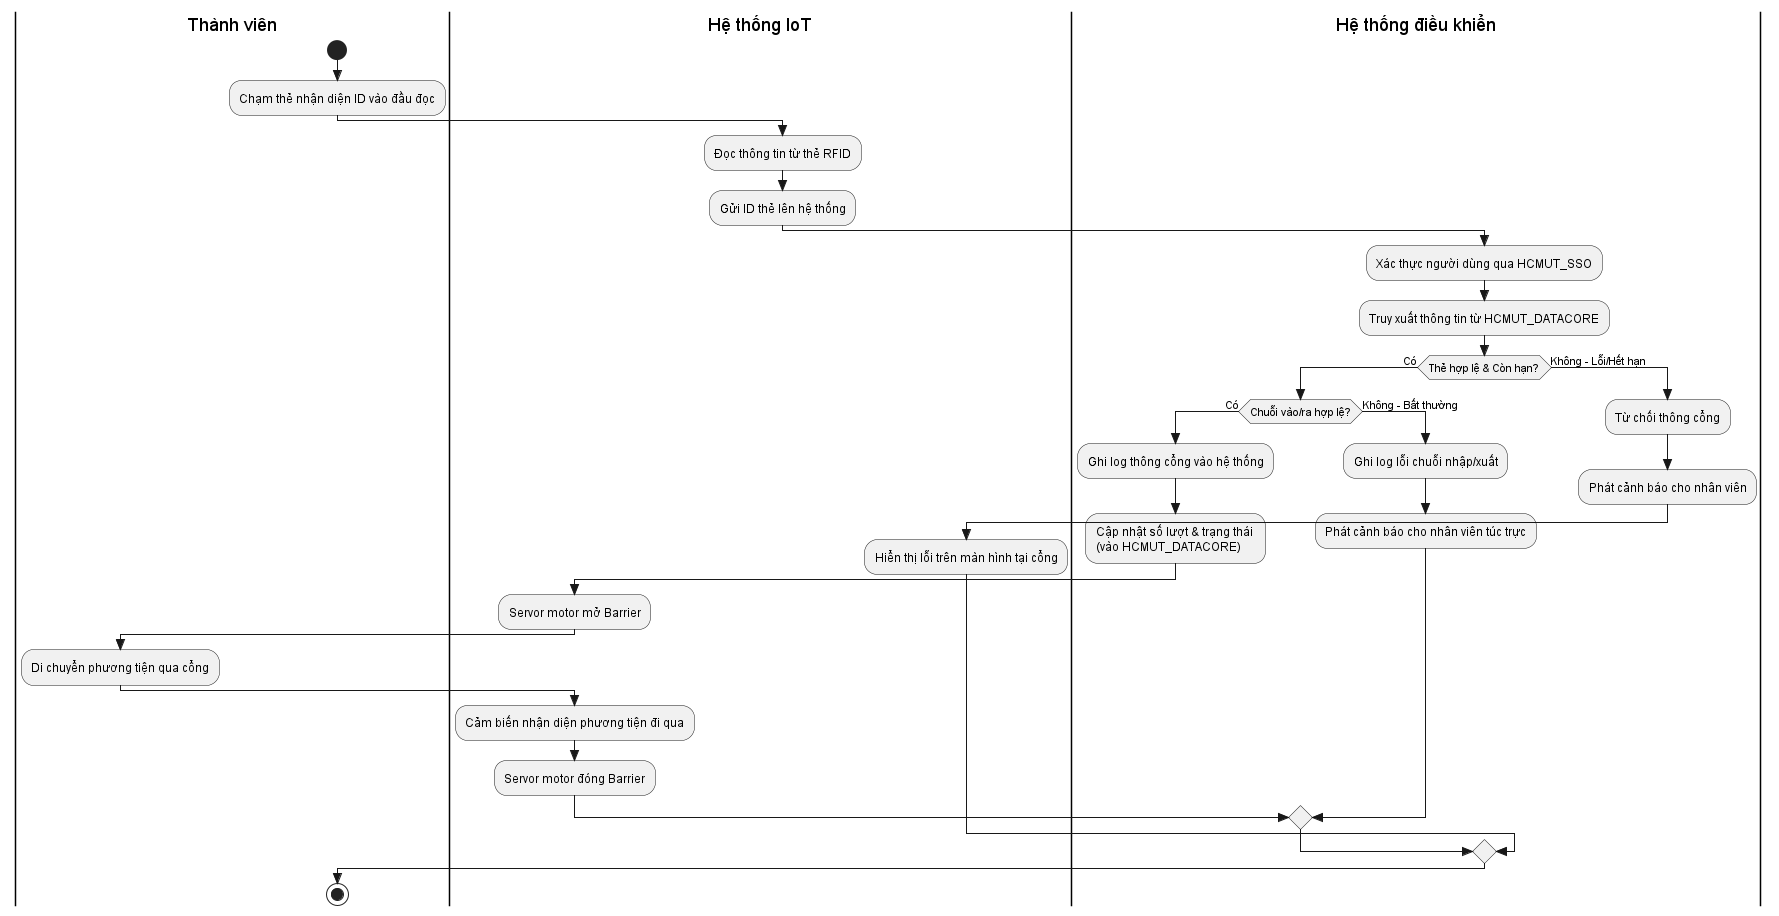
\includegraphics[angle=-90, origin=c, width=\textwidth, height=0.55\textheight, keepaspectratio]{../design/usecase-diagram/activity/mem_io.png}
    \caption{Xử lý ra/ vào cho thành viên của trường}
\end{figure}

\subsubsection{Sơ đồ trình tự (Sequence Diagram)}
\begin{figure}[htbp]
    \centering
    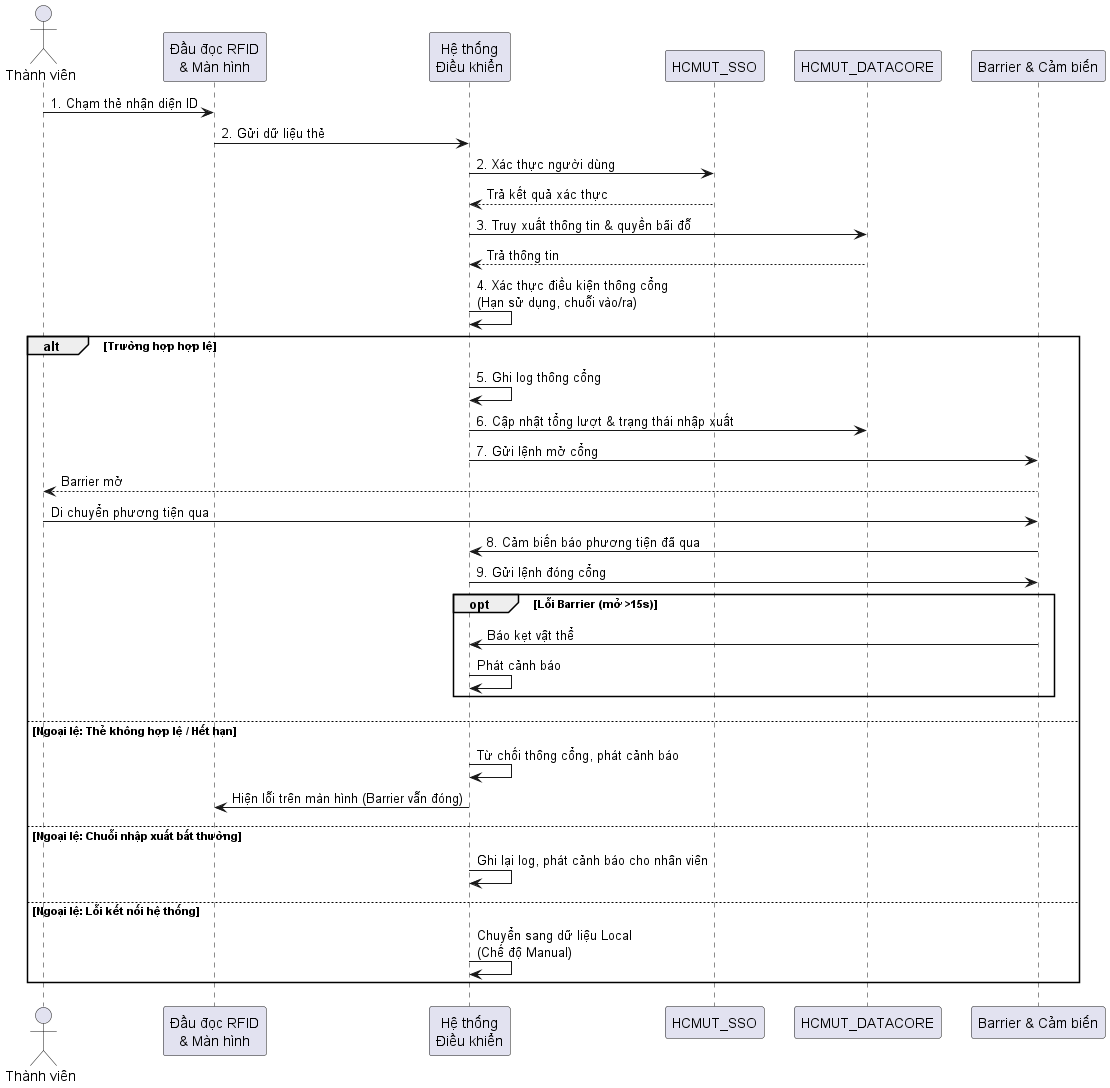
\includegraphics[angle=-90, origin=c, width=\textwidth, height=1\textheight, keepaspectratio]{../design/usecase-diagram/sequence/mem_io.png}
    \caption{Xử lý ra/ vào cho thành viên của trường}
\end{figure}

\subsection{Xử lý ra/vào cho khách vãng lai}
\subsubsection{Sơ đồ hoạt động (Activity Diagram)}
\begin{figure}[H]
    \centering
    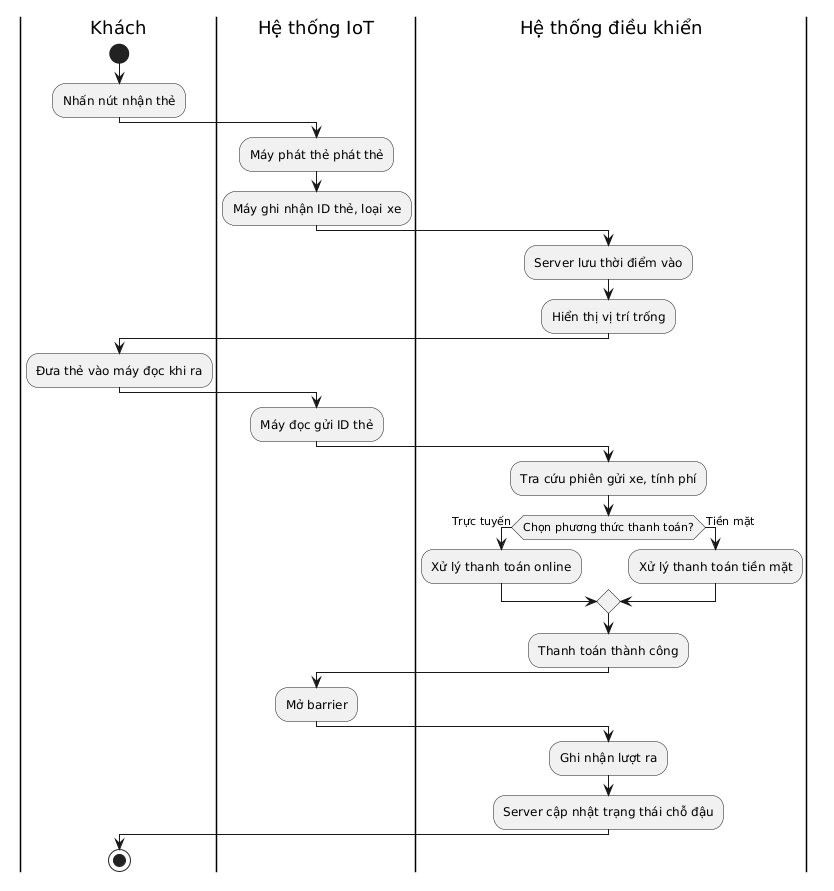
\includegraphics[width=1\textwidth, keepaspectratio]{../design/usecase-diagram/activity/guest_io.png}
    \caption{Xử lý ra/vào cho khách}
\end{figure}

\subsubsection{Sơ đồ trình tự (Sequence Diagram)}
\begin{figure}[H]
    \centering
    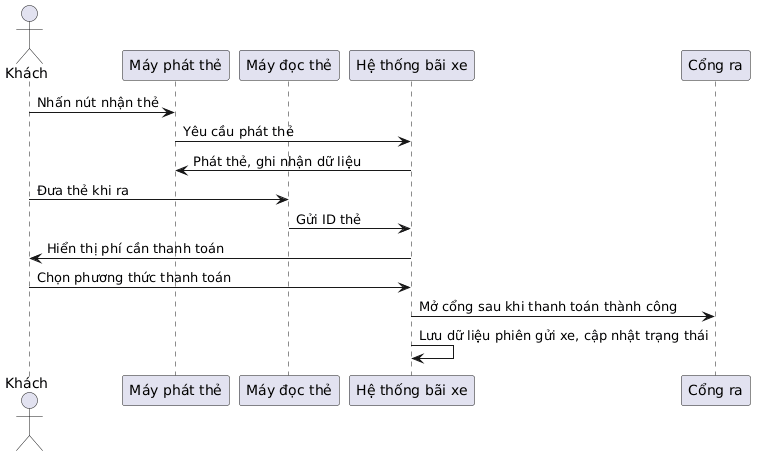
\includegraphics[angle=-90, origin=c, width=\textwidth, height=0.7\textheight, keepaspectratio]{../design/usecase-diagram/sequence/guest_io.png}
    \caption{Xử lý ra vào cho khách}
\end{figure}

\subsection{Thanh toán phí gửi xe đối với thành viên}
\subsubsection{Sơ đồ hoạt động (Activity Diagram)}
\begin{figure}[H]
    \centering
    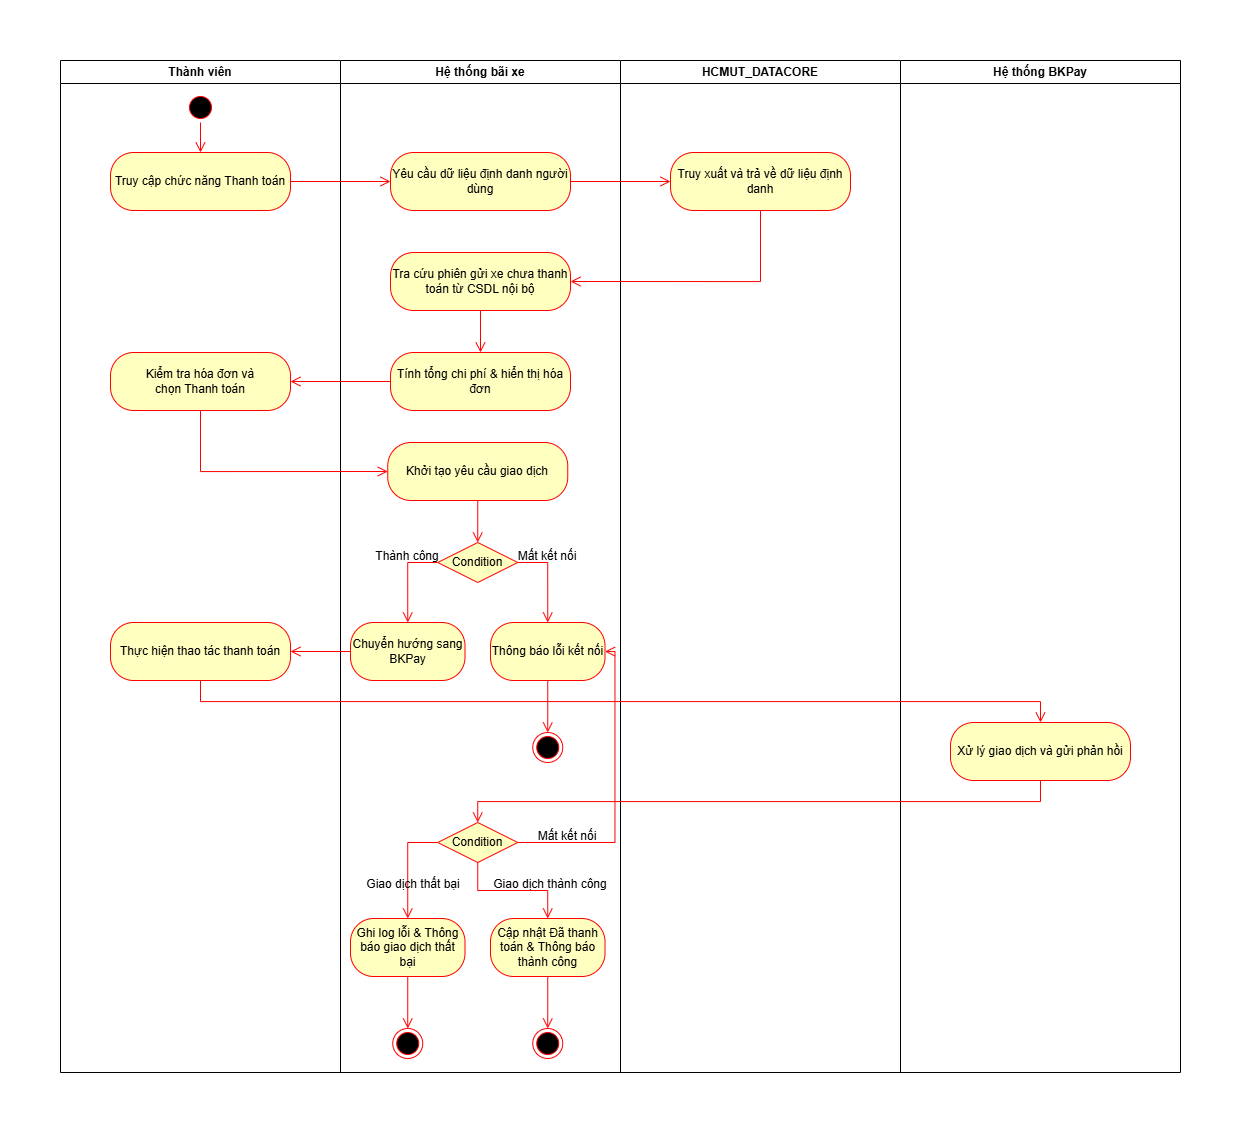
\includegraphics[width=\textwidth, keepaspectratio]{../design/usecase-diagram/activity/mem_pay.png}
    \caption{Activity Diagram - Thành viên thanh toán phí}
\end{figure}

\subsubsection{Sơ đồ trình tự (Sequence Diagram)}
\begin{figure}[H]
    \centering
    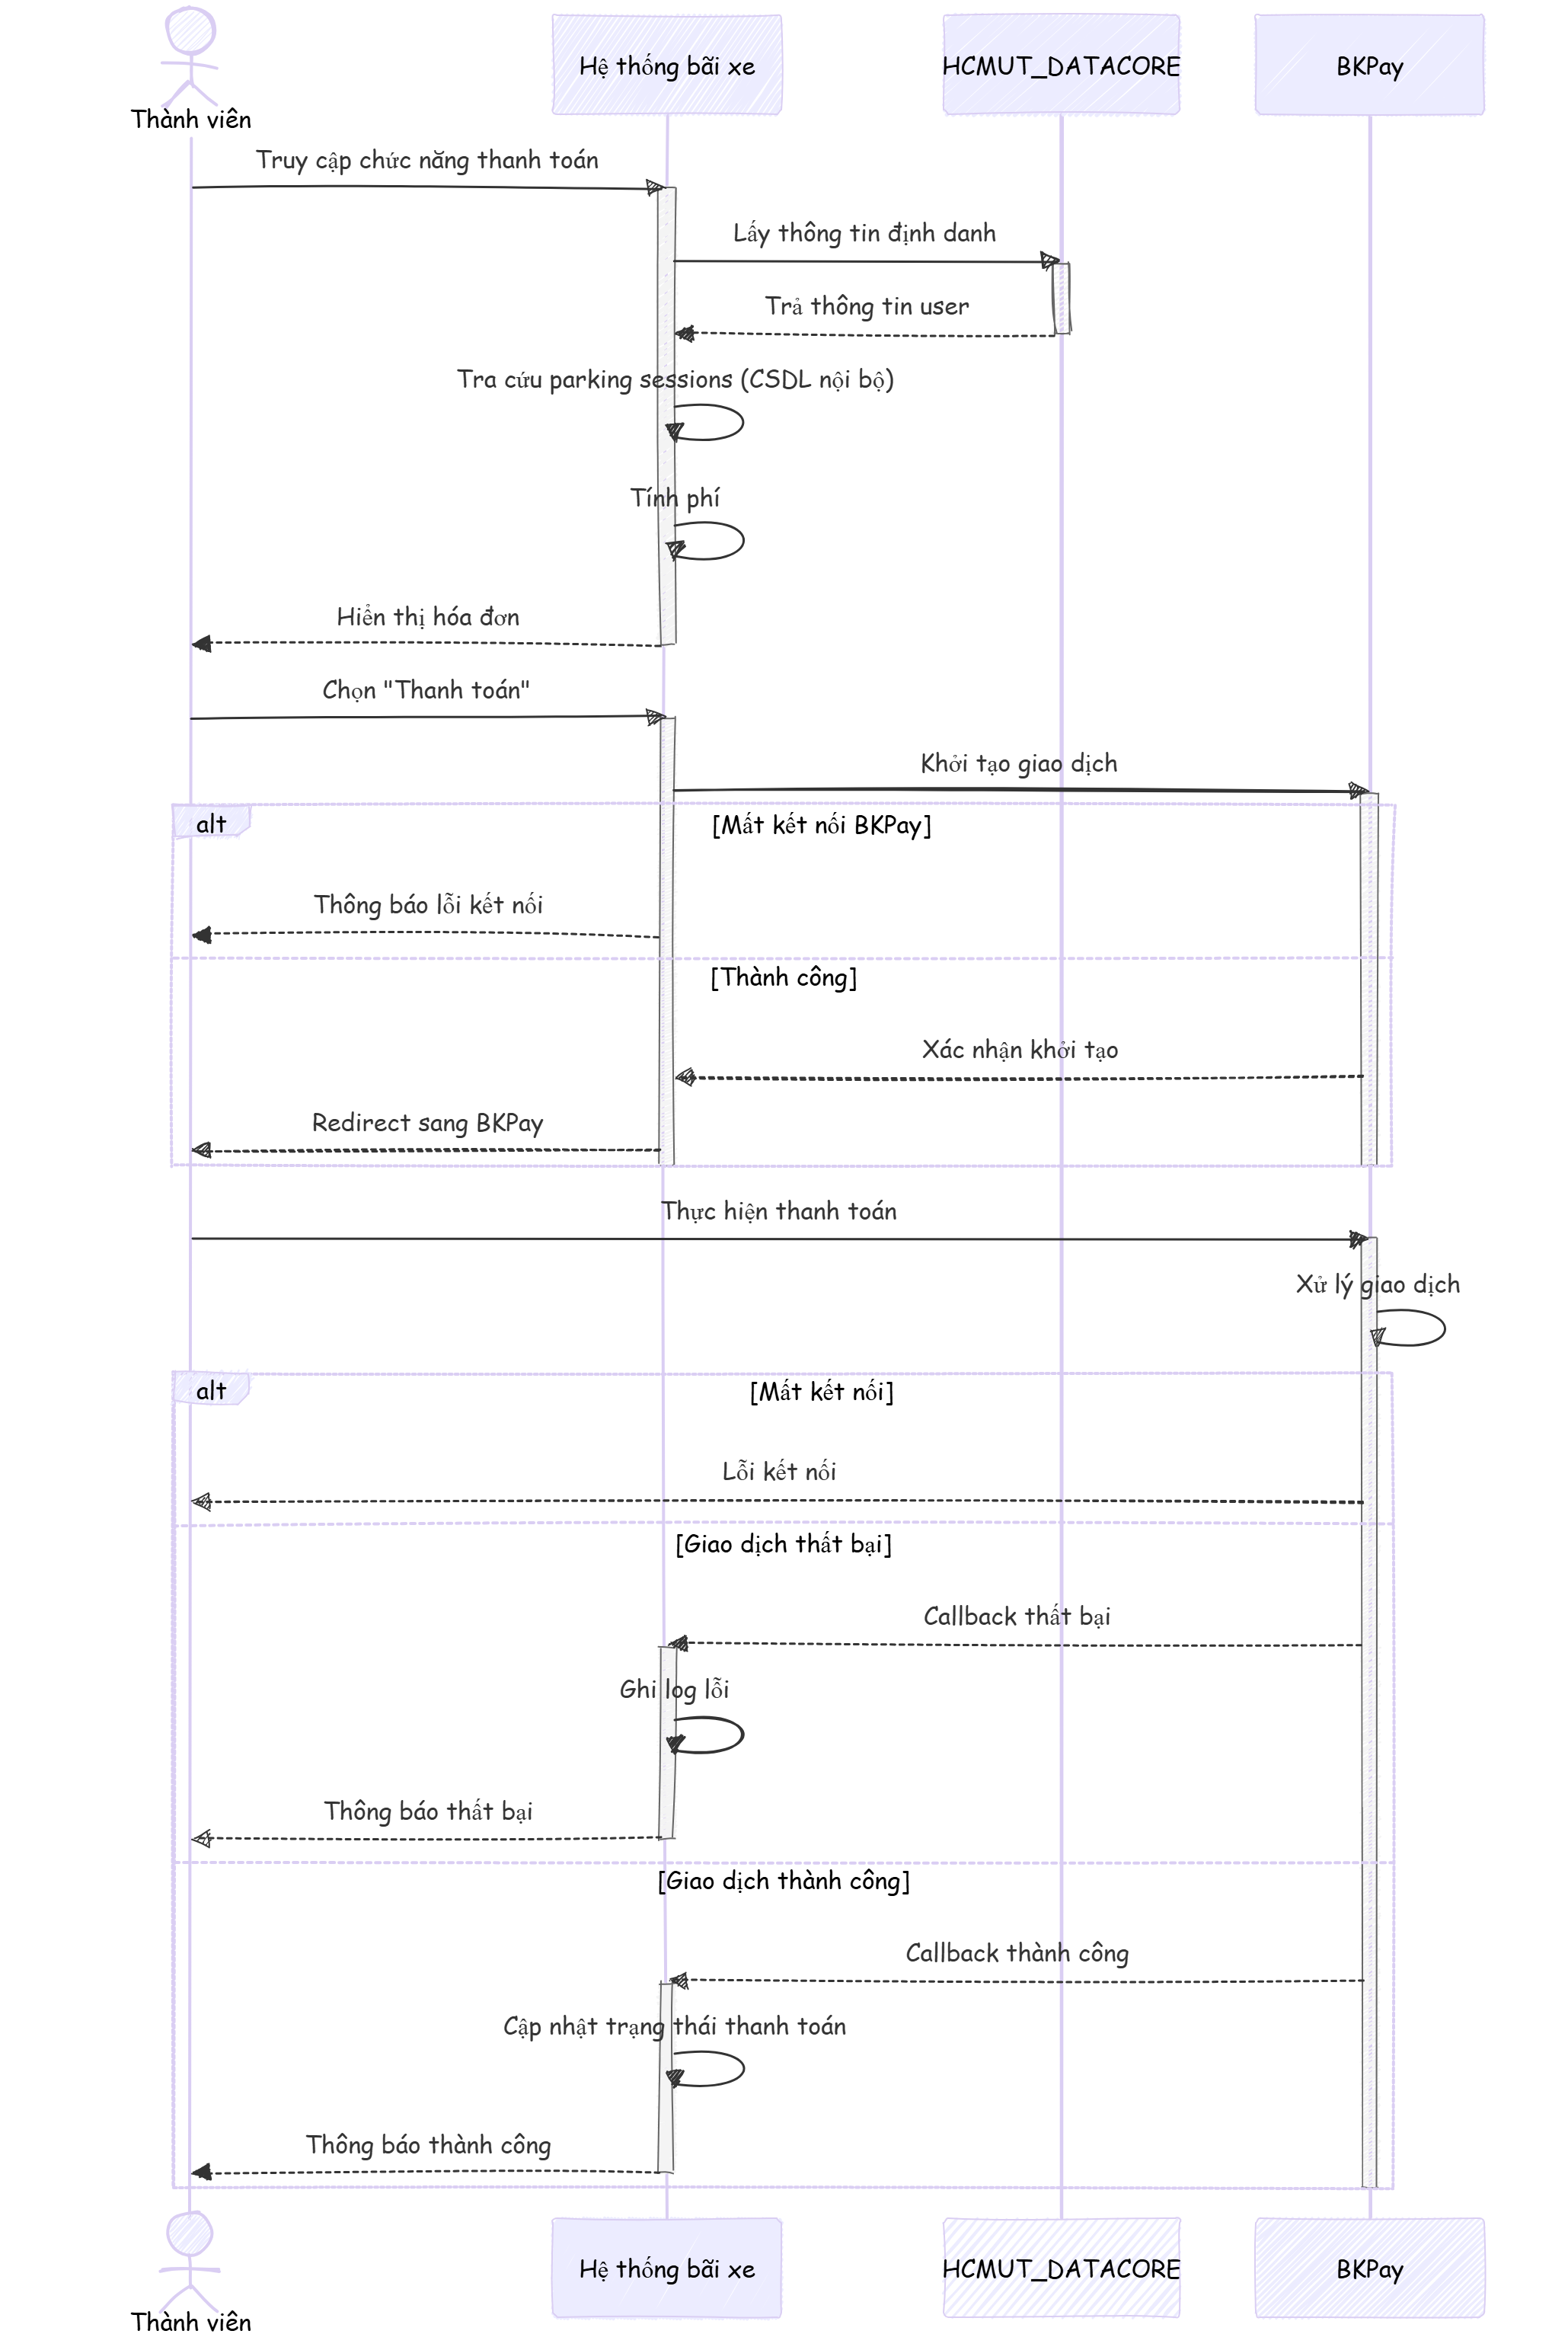
\includegraphics[width=0.9\textwidth, height=0.9\textheight, keepaspectratio]{../design/usecase-diagram/sequence/mem_pay.png}
    \caption{Sequence Diagram - Thành viên thanh toán phí}
\end{figure}

\subsection{Thanh toán phí gửi xe cho khách vãng lai}
\subsubsection{Sơ đồ hoạt động (Activity Diagram)}
\begin{figure}[H]
    \centering
    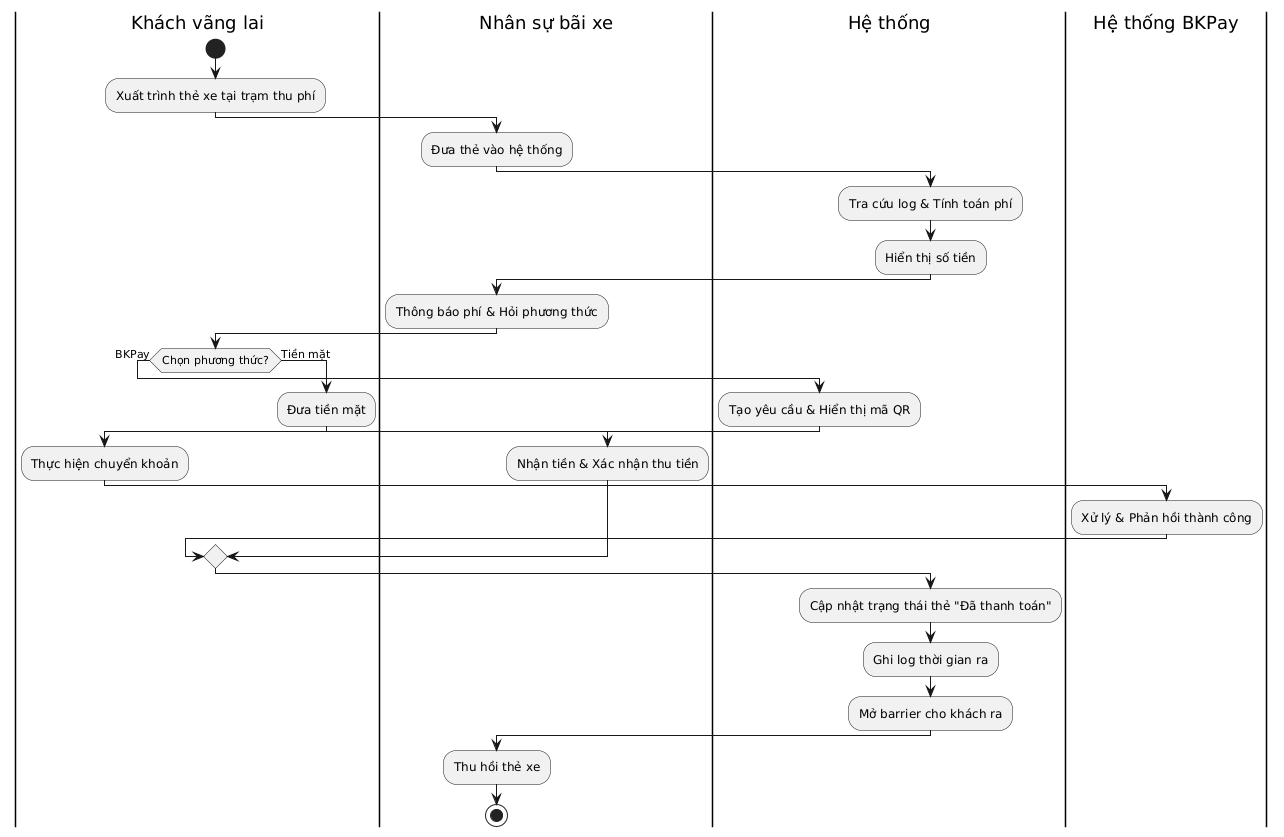
\includegraphics[angle=-90, width=0.5\textheight, keepaspectratio]{../design/usecase-diagram/activity/guest_pay_Ordinary.png}
    \caption{Thanh toán phí gửi xe cho khách (Luồng thông thường)}
\end{figure}

\begin{figure}[H]
    \centering
    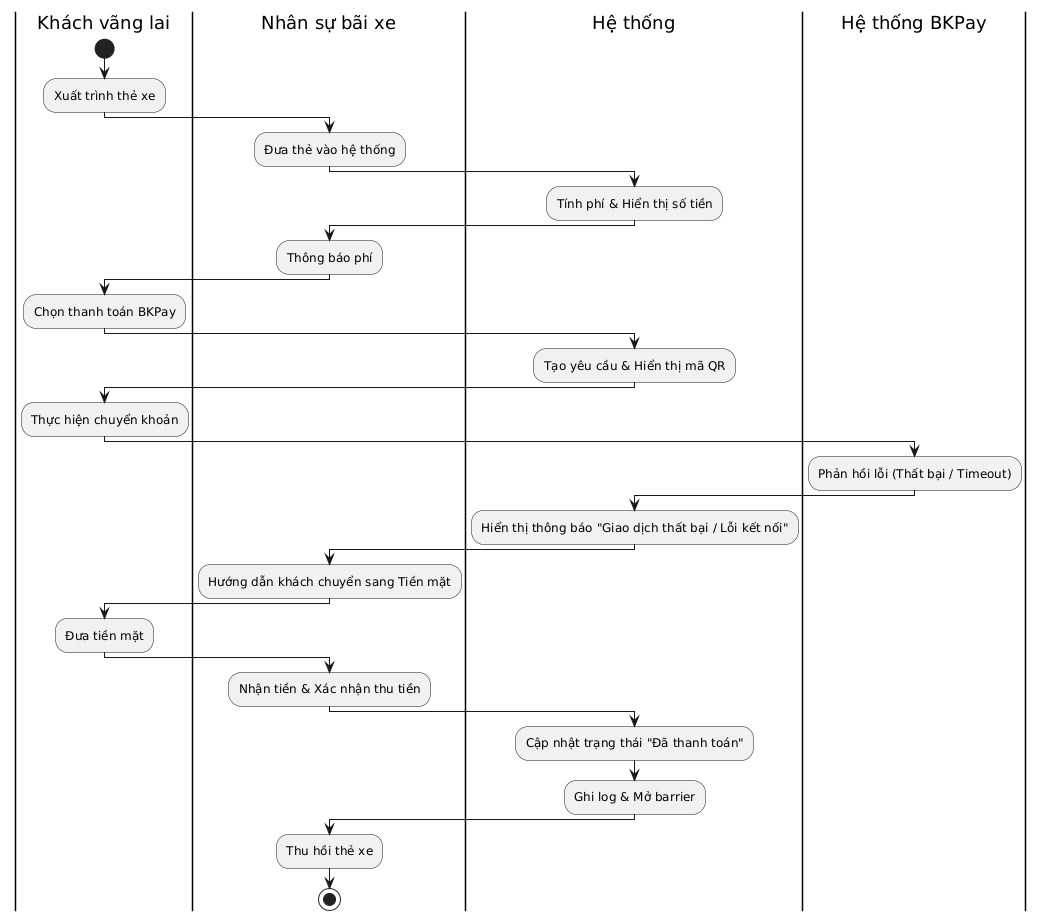
\includegraphics[angle=-90, width=0.6\textheight, keepaspectratio]{../design/usecase-diagram/activity/guest_pay_BKPayFailed.png}
    \caption{Thanh toán phí gửi xe cho khách (BKPay gặp lỗi)}
\end{figure}

\begin{figure}[H]
    \centering
    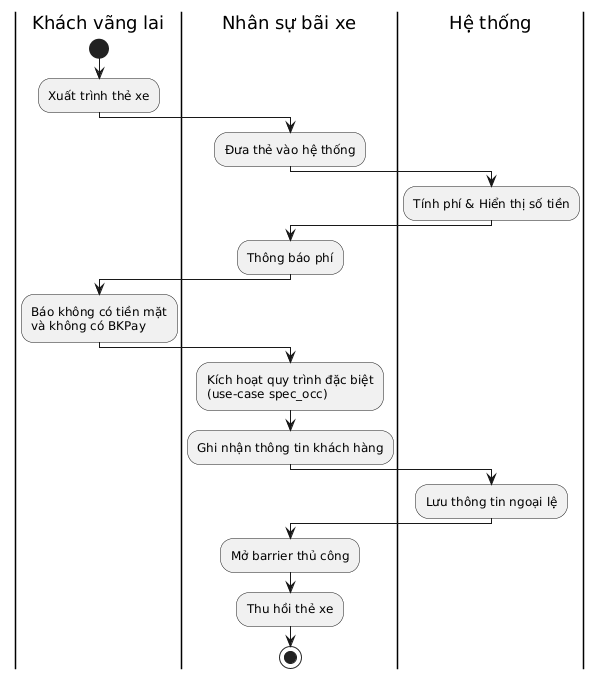
\includegraphics[width=0.9\textwidth, keepaspectratio]{../design/usecase-diagram/activity/guest_pay_NoCashAndNoBKPay.png}
    \caption{Thanh toán phí gửi xe cho khách (Không tiền mặt và không BKPay)}
\end{figure}

\begin{figure}[H]
    \centering
    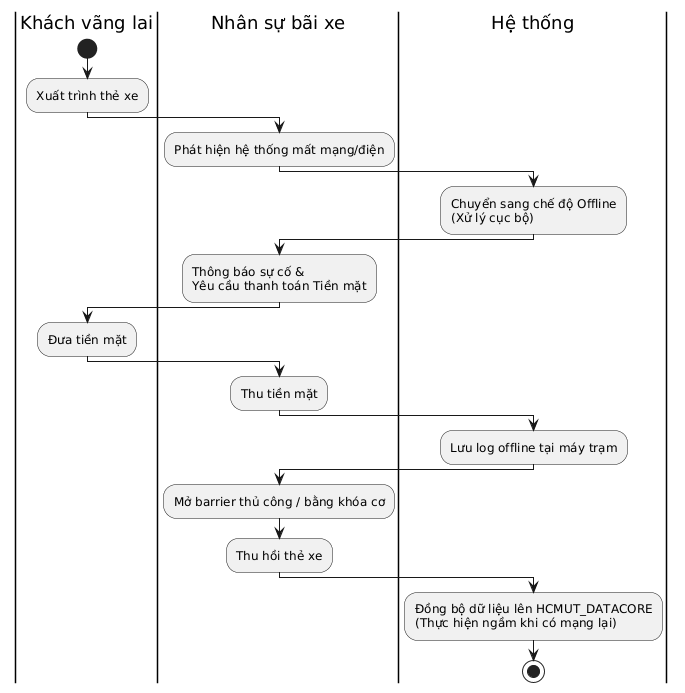
\includegraphics[width=0.9\textwidth, keepaspectratio]{../design/usecase-diagram/activity/guest_pay_NoConnection.png}
    \caption{Thanh toán phí gửi xe cho khách (Bãi xe tạm ngắt hệ thống)}
\end{figure}

\subsubsection{Sơ đồ trình tự (Sequence Diagram)}
\begin{figure}[H]
    \centering
    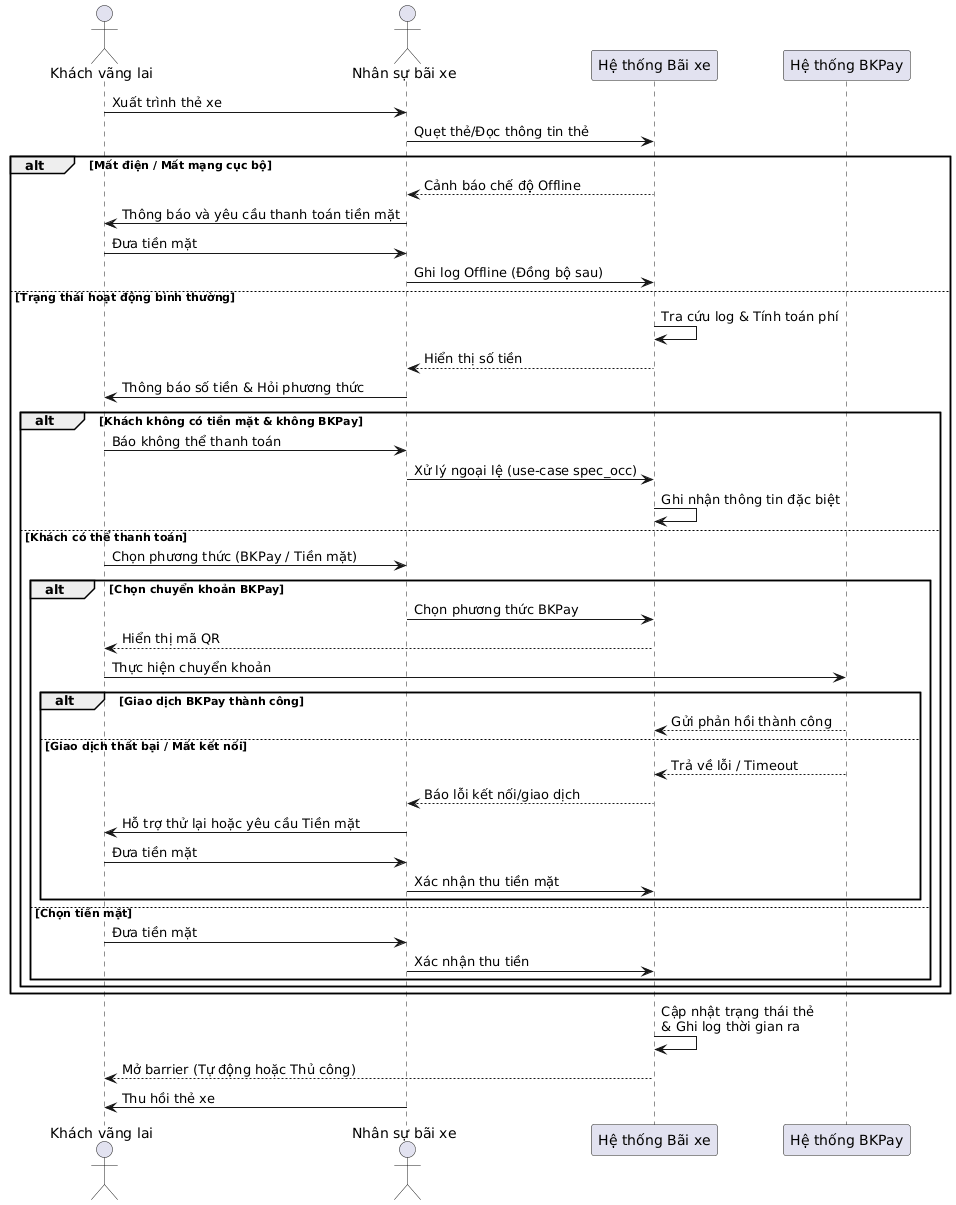
\includegraphics[width=\textwidth, height=0.9\textheight, keepaspectratio]{../design/usecase-diagram/sequence/guest_pay_sequence_diagram.png}
    \caption{Thanh toán phí gửi xe cho khách}
\end{figure}

\subsection{Quản lý chi phí gửi xe}
\subsubsection{Sơ đồ hoạt động (Activity Diagram)}
\begin{figure}[H]
    \centering
    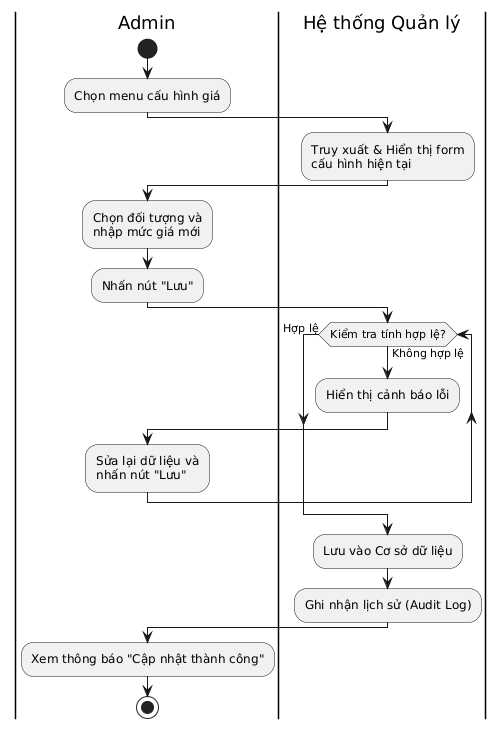
\includegraphics[width=0.8\textwidth, keepaspectratio]{../design/usecase-diagram/activity/ad_price.png}
    \caption{Quản lý chi phí gửi xe}
\end{figure}

\subsubsection{Sơ đồ trình tự (Sequence Diagram)}
\begin{figure}[H]
    \centering
    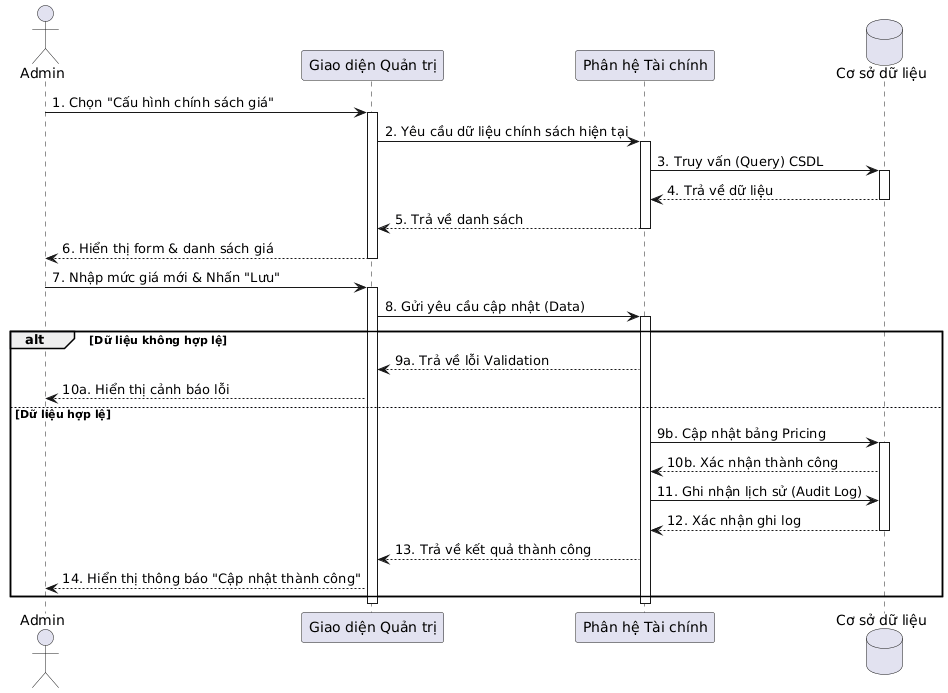
\includegraphics[angle=-90, origin=c, width=\textwidth, height=0.7\textheight, keepaspectratio]{../design/usecase-diagram/sequence/ad_price.png}
    \caption{Quản lý chi phí gửi xe}
\end{figure}

\subsection{Quản lý nhân sự}
\subsubsection{Sơ đồ hoạt động (Activity Diagram)}
\begin{figure}[H]
    \centering
    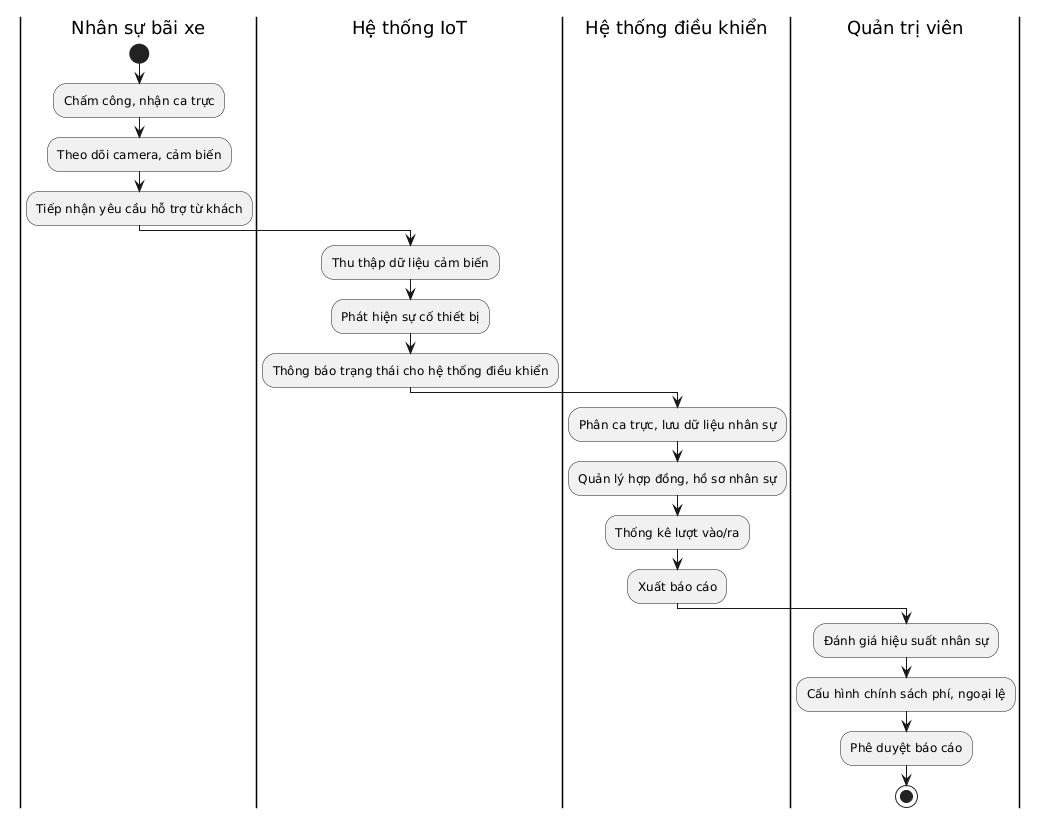
\includegraphics[width=\textwidth, keepaspectratio]{../design/usecase-diagram/activity/ad_hr.png}
    \caption{Quản lý nhân sự}
\end{figure}

\subsubsection{Sơ đồ trình tự (Sequence Diagram)}
\begin{figure}[H]
    \centering
    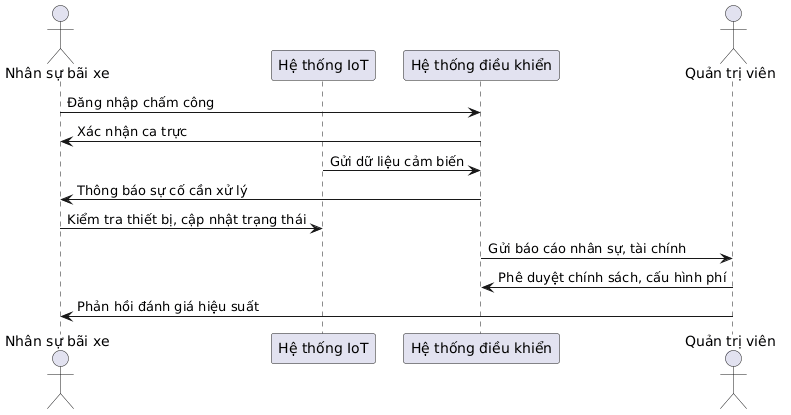
\includegraphics[angle=-90, origin=c, width=\textwidth, height=0.65\textheight, keepaspectratio]{../design/usecase-diagram/sequence/ad_hr.png}
    \caption{Quản lý nhân sự}
\end{figure}

\subsection{Truy vấn lịch sử ra vào bãi đỗ xe}
\subsubsection{Sơ đồ hoạt động (Activity Diagram)}
\begin{figure}[H]
    \centering
    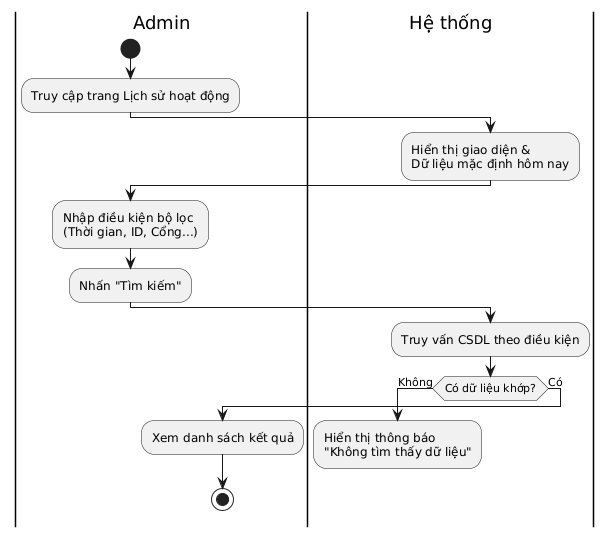
\includegraphics[width=\textwidth, keepaspectratio]{../design/usecase-diagram/activity/ad_his.png}
    \caption{Truy vấn lịch sử ra vào bãi đỗ xe}
\end{figure}

\subsubsection{Sơ đồ trình tự (Sequence Diagram)}
\begin{figure}[H]
    \centering
    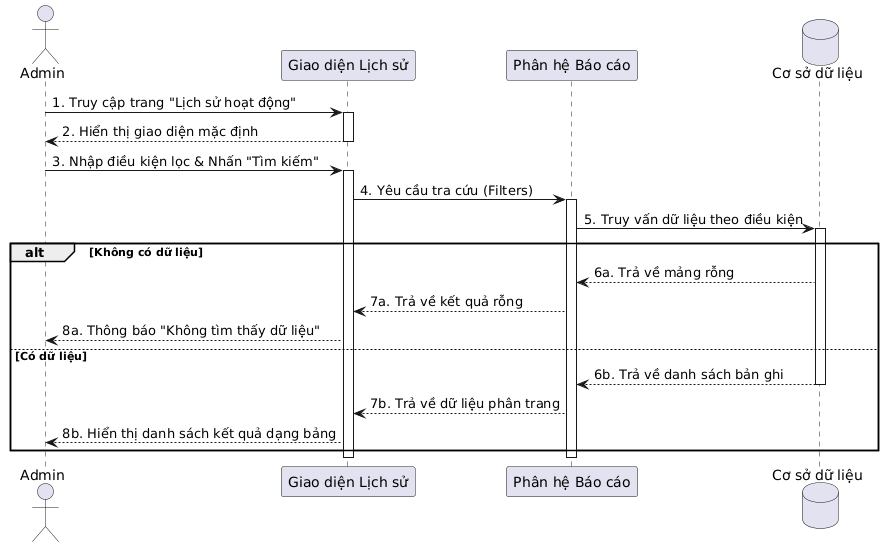
\includegraphics[angle=-90, origin=c, width=\textwidth, height=0.7\textheight, keepaspectratio]{../design/usecase-diagram/sequence/ad_his.png}
    \caption{Truy vấn lịch sử ra vào bãi đỗ xe}
\end{figure}

\subsection{Kiểm soát về số lượng và vị trí chỗ trống}
\subsubsection{Sơ đồ hoạt động (Activity Diagram)}
\begin{figure}[H]
    \centering
    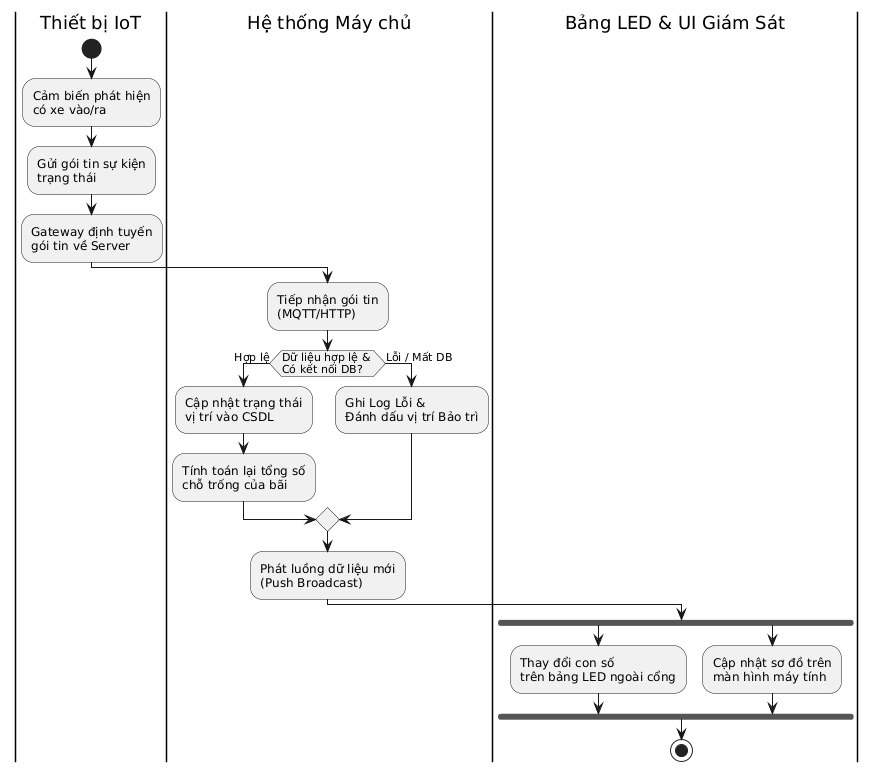
\includegraphics[width=0.9\textwidth, keepaspectratio]{../design/usecase-diagram/activity/iot.png}
    \caption{Kiểm soát về số lượng và vị trí chỗ trống}
\end{figure}

\subsubsection{Sơ đồ trình tự (Sequence Diagram)}
\begin{figure}[H]
    \centering
    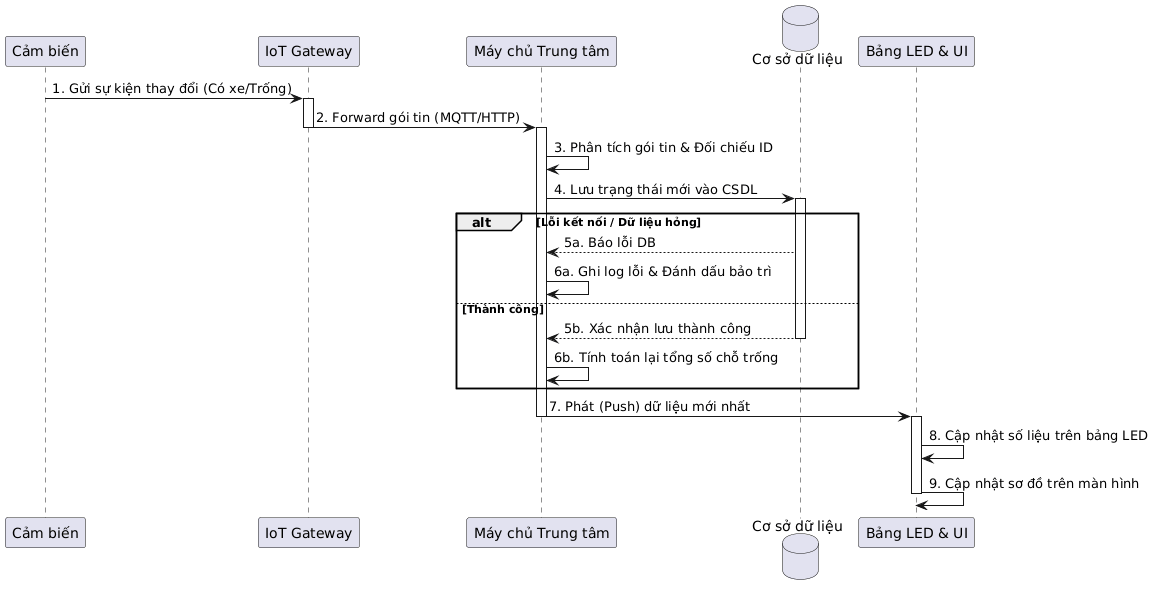
\includegraphics[angle=-90, origin=c, width=\textwidth, height=0.65\textheight, keepaspectratio]{../design/usecase-diagram/sequence/iot.png}
    \caption{Kiểm soát về số lượng và vị trí chỗ trống}
\end{figure}

\subsection{Xử lý trường hợp đặc biệt - cháy nổ}
\subsubsection{Sơ đồ hoạt động (Activity Diagram)}
\begin{figure}[H]
    \centering
    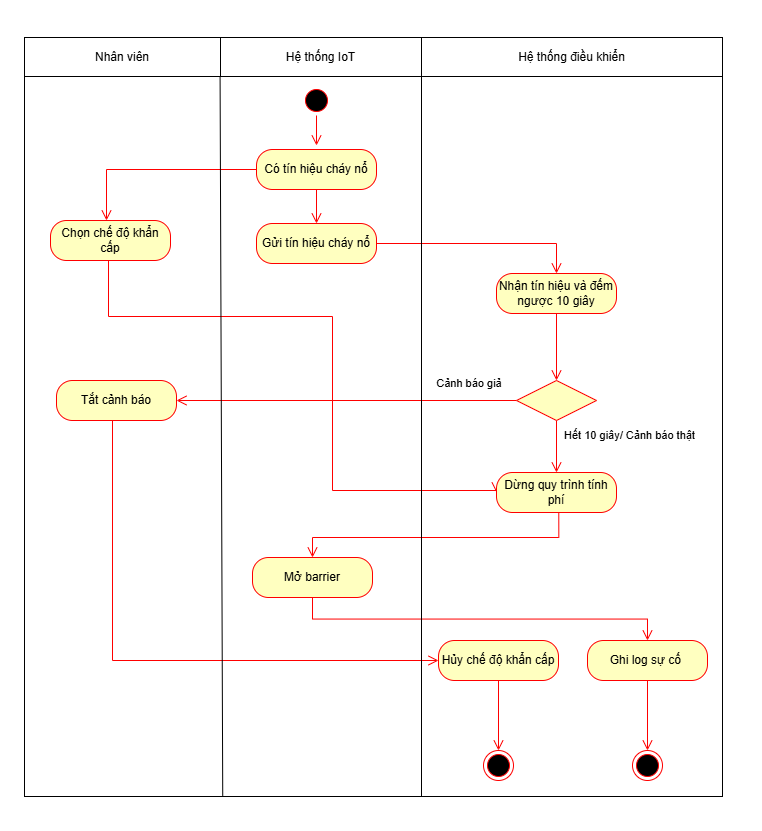
\includegraphics[width=0.9\textwidth, keepaspectratio]{../design/usecase-diagram/activity/activate_emergency_mode.png}
    \caption{Xử lý trường hợp đặc biệt - cháy nổ}
\end{figure}

\subsubsection{Sơ đồ trình tự (Sequence Diagram)}
\begin{figure}[H]
    \centering
    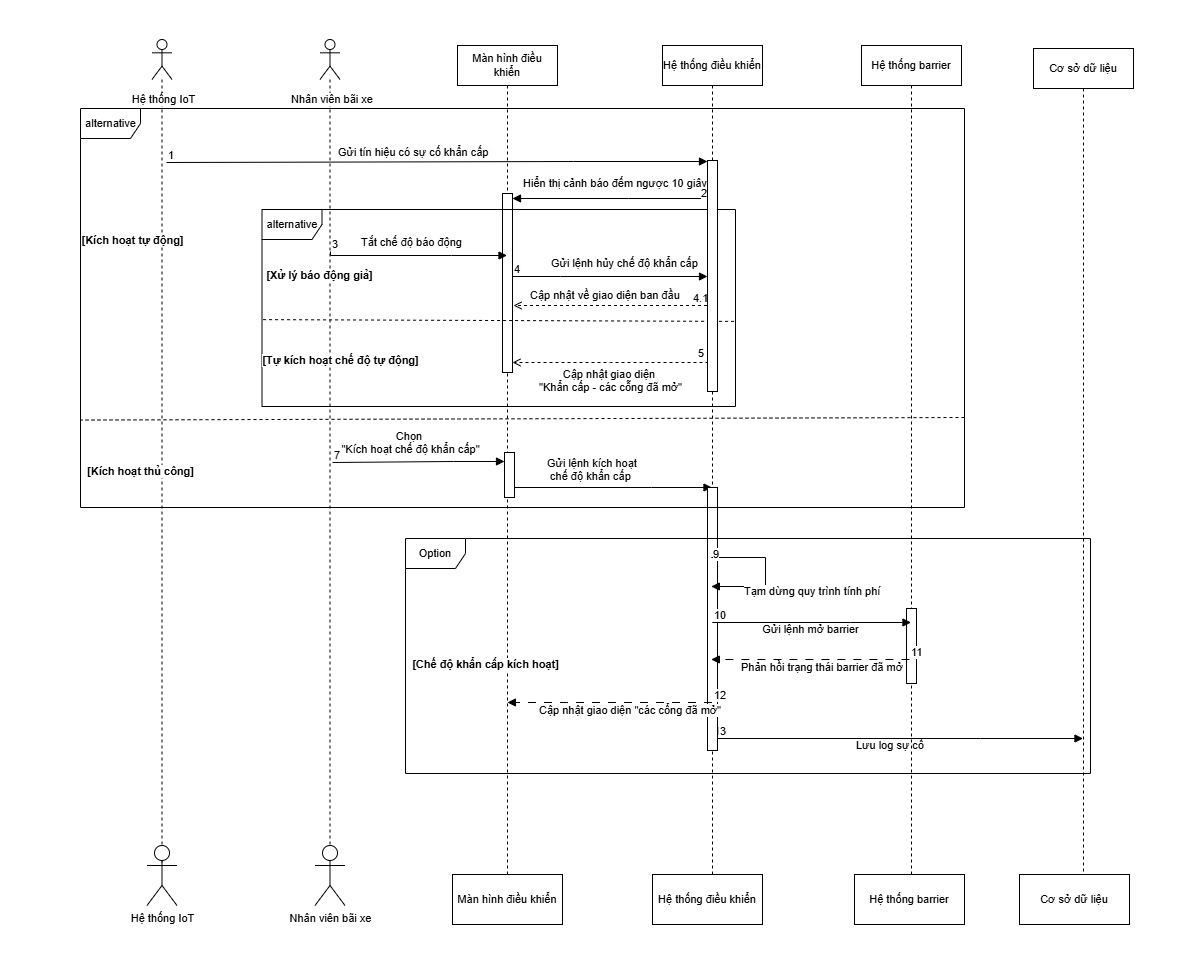
\includegraphics[angle=-90, origin=c, width=\textwidth, height=0.9\textheight, keepaspectratio]{../design/usecase-diagram/sequence/activate_emergency_mode.png}
    \caption{Xử lý trường hợp đặc biệt - cháy nổ}
\end{figure}

\subsection{Xử lý trường hợp đặc biệt - lỗi thanh toán của khách}
\subsubsection{Sơ đồ hoạt động (Activity Diagram)}
\begin{figure}[H]
    \centering
    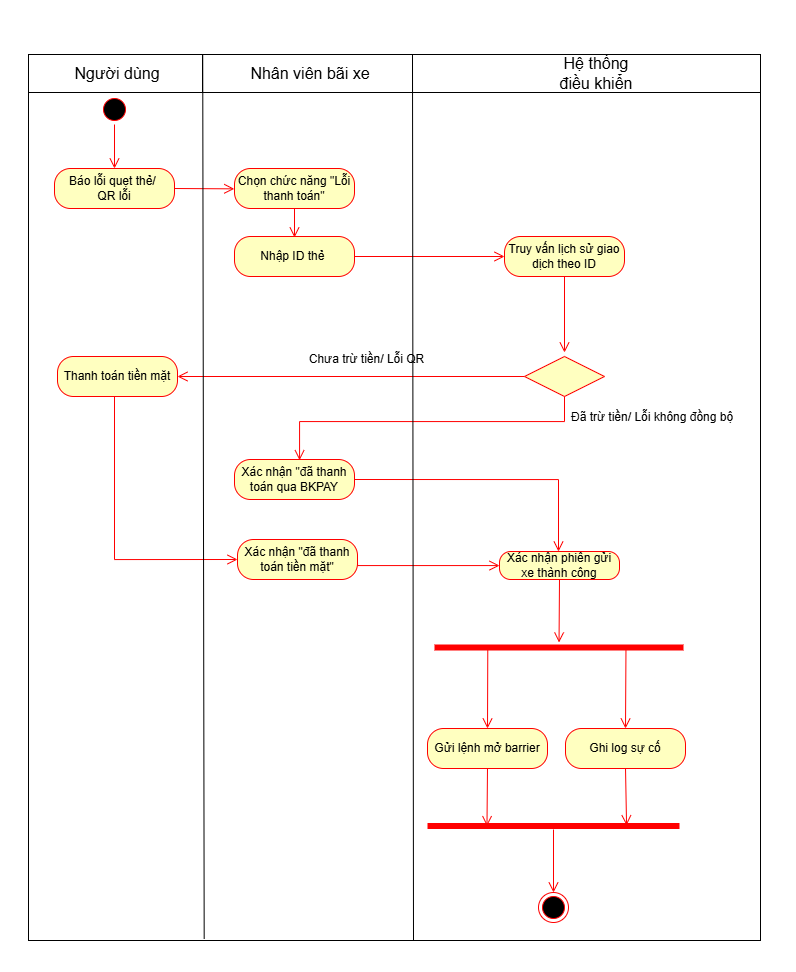
\includegraphics[width=0.9\textwidth, keepaspectratio]{../design/usecase-diagram/activity/quest_payment_error.png}
    \caption{Xử lý trường hợp đặc biệt - lỗi thanh toán của khách}
\end{figure}

\subsubsection{Sơ đồ trình tự (Sequence Diagram)}
\begin{figure}[H]
    \centering
    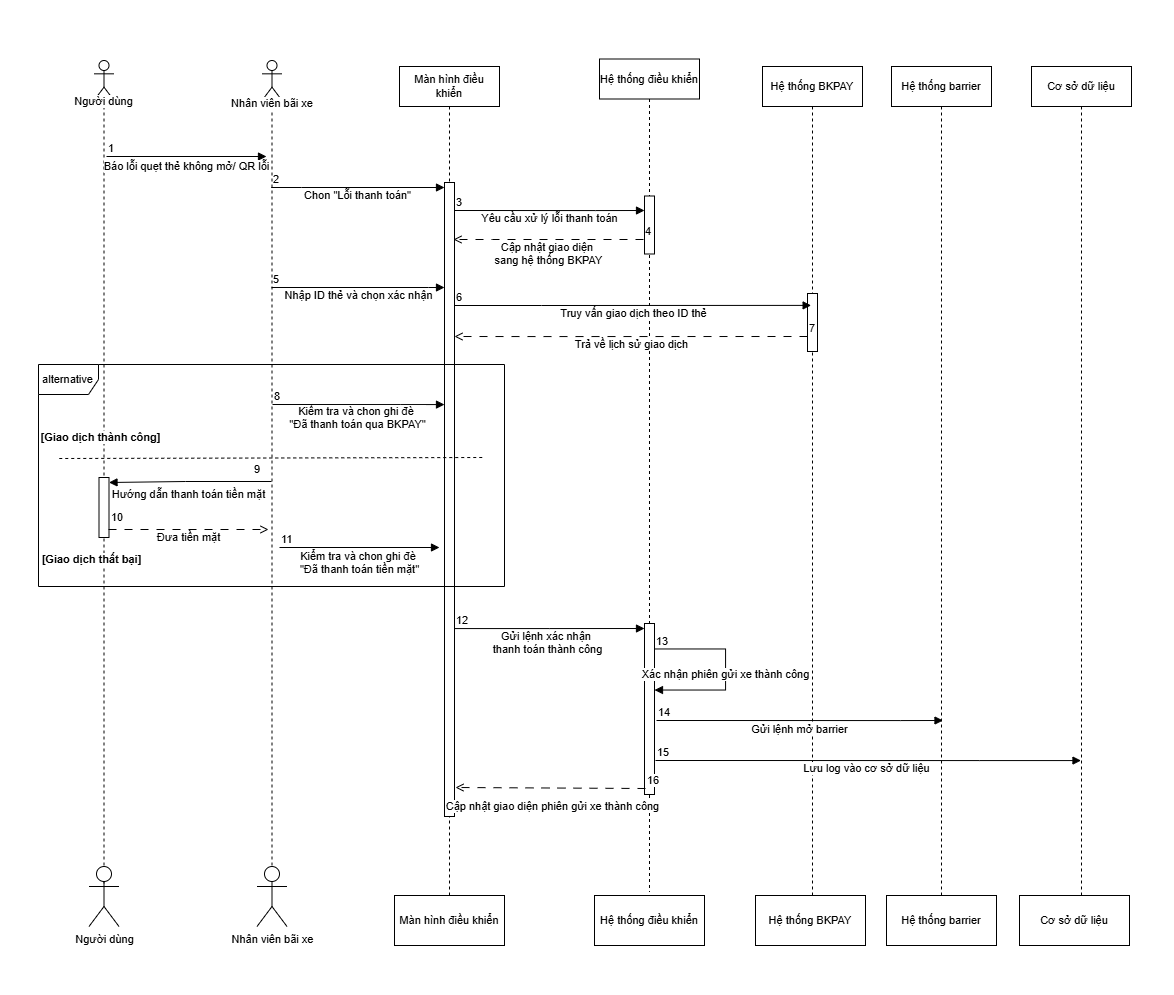
\includegraphics[angle=-90, origin=c, width=\textwidth, height=0.9\textheight, keepaspectratio]{../design/usecase-diagram/sequence/quest_payment_error.png}
    \caption{Xử lý trường hợp đặc biệt - lỗi thanh toán của khách}
\end{figure}

\subsection{Xử lý trường hợp đặc biệt - thành viên trường quên thẻ}
\subsubsection{Sơ đồ hoạt động (Activity Diagram)}
\begin{figure}[H]
    \centering
    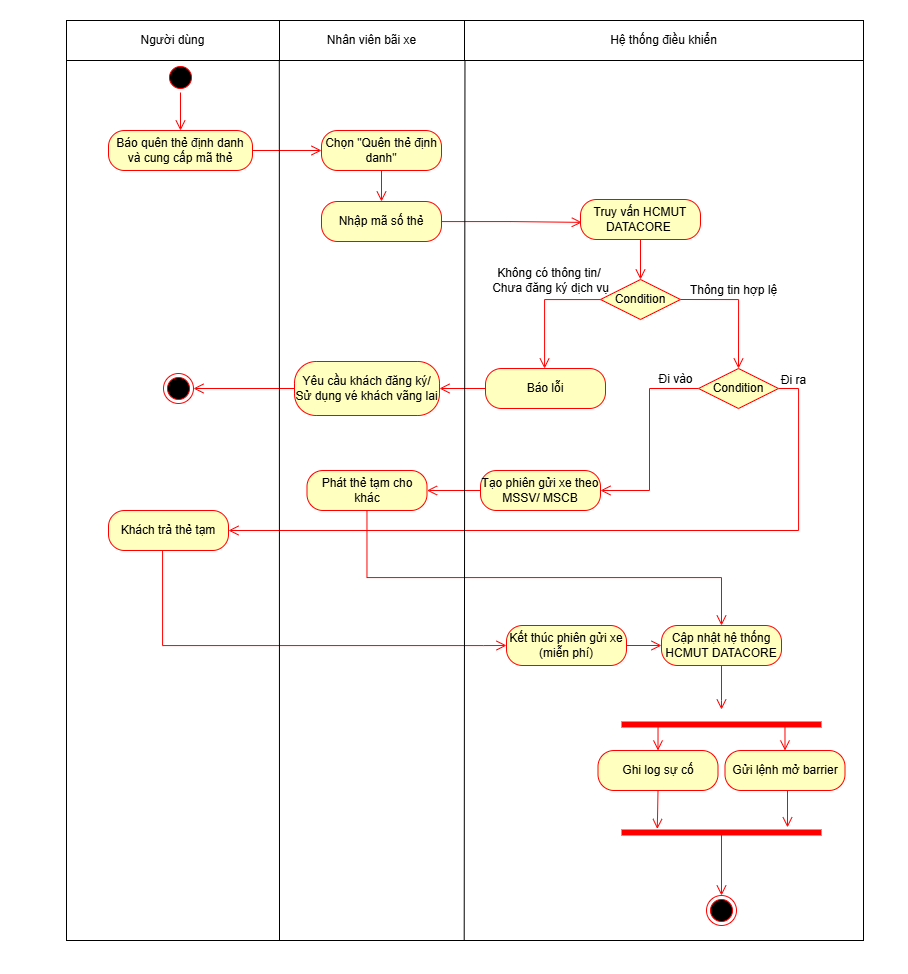
\includegraphics[width=0.9\textwidth, keepaspectratio]{../design/usecase-diagram/activity/foget_id_card.png}
    \caption{Xử lý trường hợp đặc biệt - thành viên trường quên thẻ (được xử lý giống khách)}
\end{figure}

\subsubsection{Sơ đồ trình tự (Sequence Diagram)}
\begin{figure}[H]
    \centering
    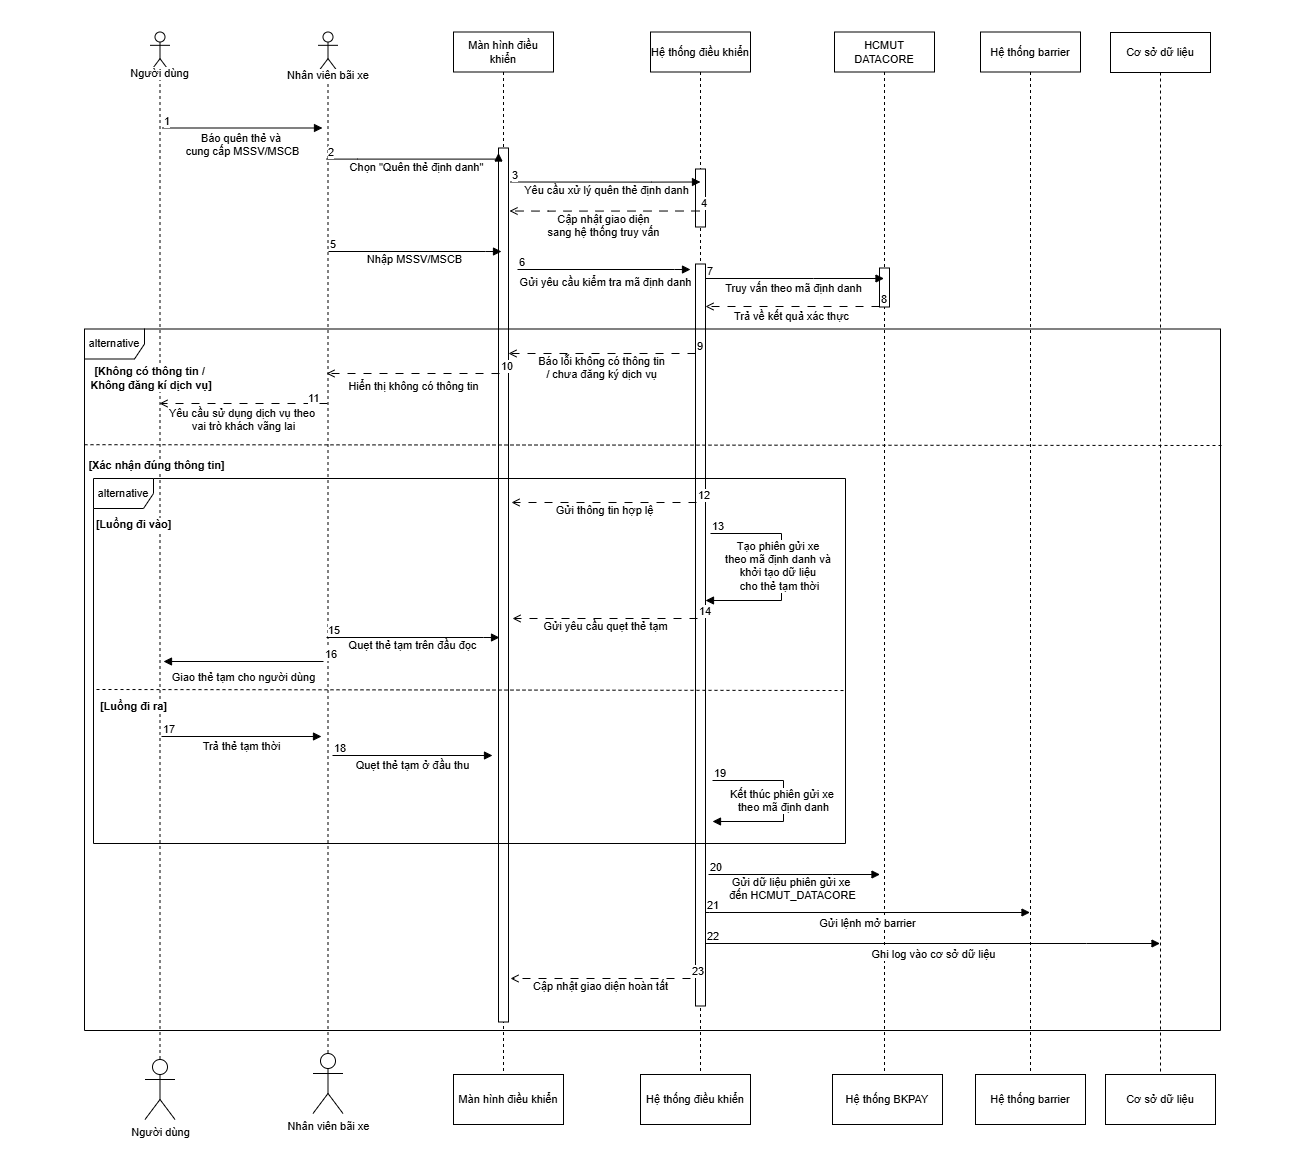
\includegraphics[angle=-90, origin=c, width=\textwidth, height=0.9\textheight, keepaspectratio]{../design/usecase-diagram/sequence/foget_id_card.png}
    \caption{Xử lý trường hợp đặc biệt - thành viên trường quên thẻ (được xử lý giống khách)}
\end{figure}

\subsection{Xử lý trường hợp đặc biệt - mất thẻ}
\subsubsection{Sơ đồ hoạt động (Activity Diagram)}
\begin{figure}[H]
    \centering
    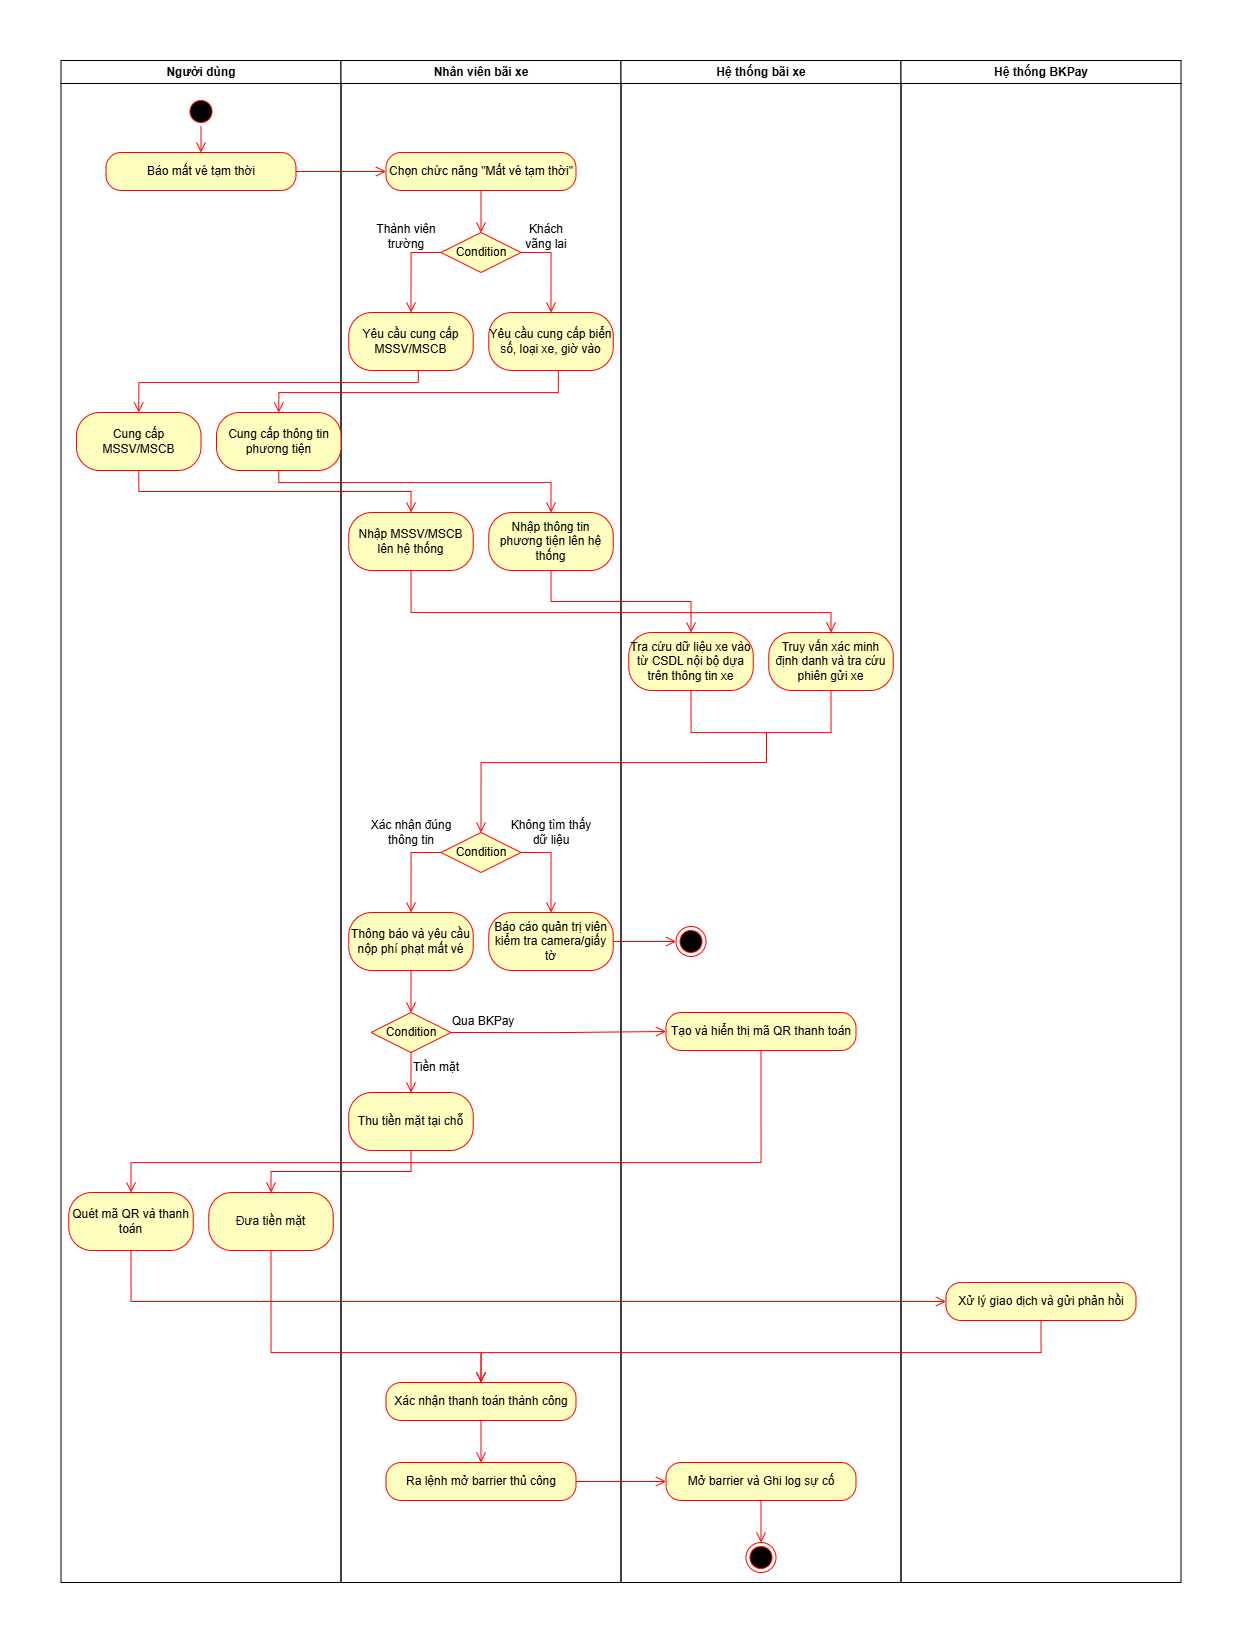
\includegraphics[width=0.9\textwidth, keepaspectratio]{../design/usecase-diagram/activity/lost_temp_card.png}
    \caption{Xử lý trường hợp đặc biệt - mất thẻ}
\end{figure}

\subsubsection{Sơ đồ trình tự (Sequence Diagram)}
\begin{figure}[H]
    \centering
    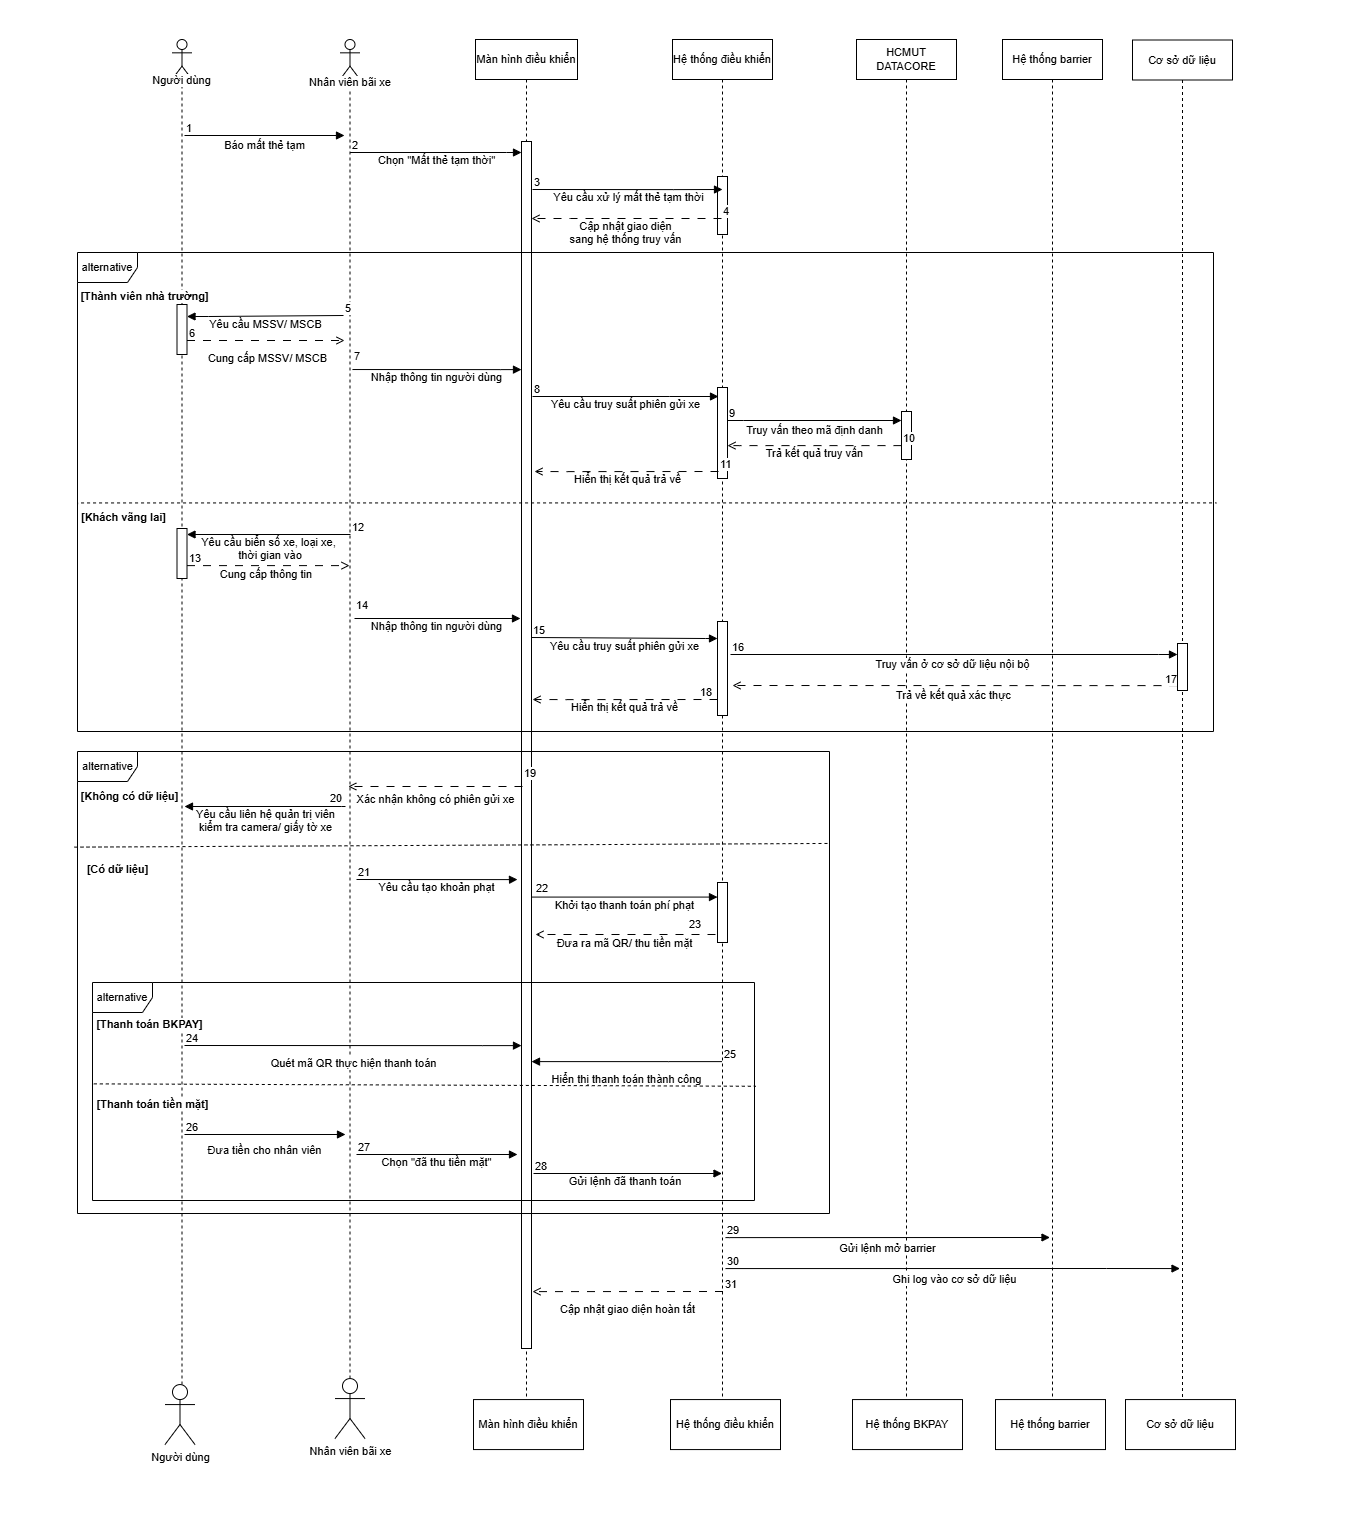
\includegraphics[width=\textwidth, keepaspectratio]{../design/usecase-diagram/sequence/lost_temp_card.png}
    \caption{Xử lý trường hợp đặc biệt - mất thẻ}
\end{figure}


% overdue_card là spec_occ_5

\subsection{Xử lý trường hợp đặc biệt-thẻ quá hạn}
\subsubsection{Sơ đồ hoạt động (Activity Diagram)}
\begin{figure}[H]
    \centering
    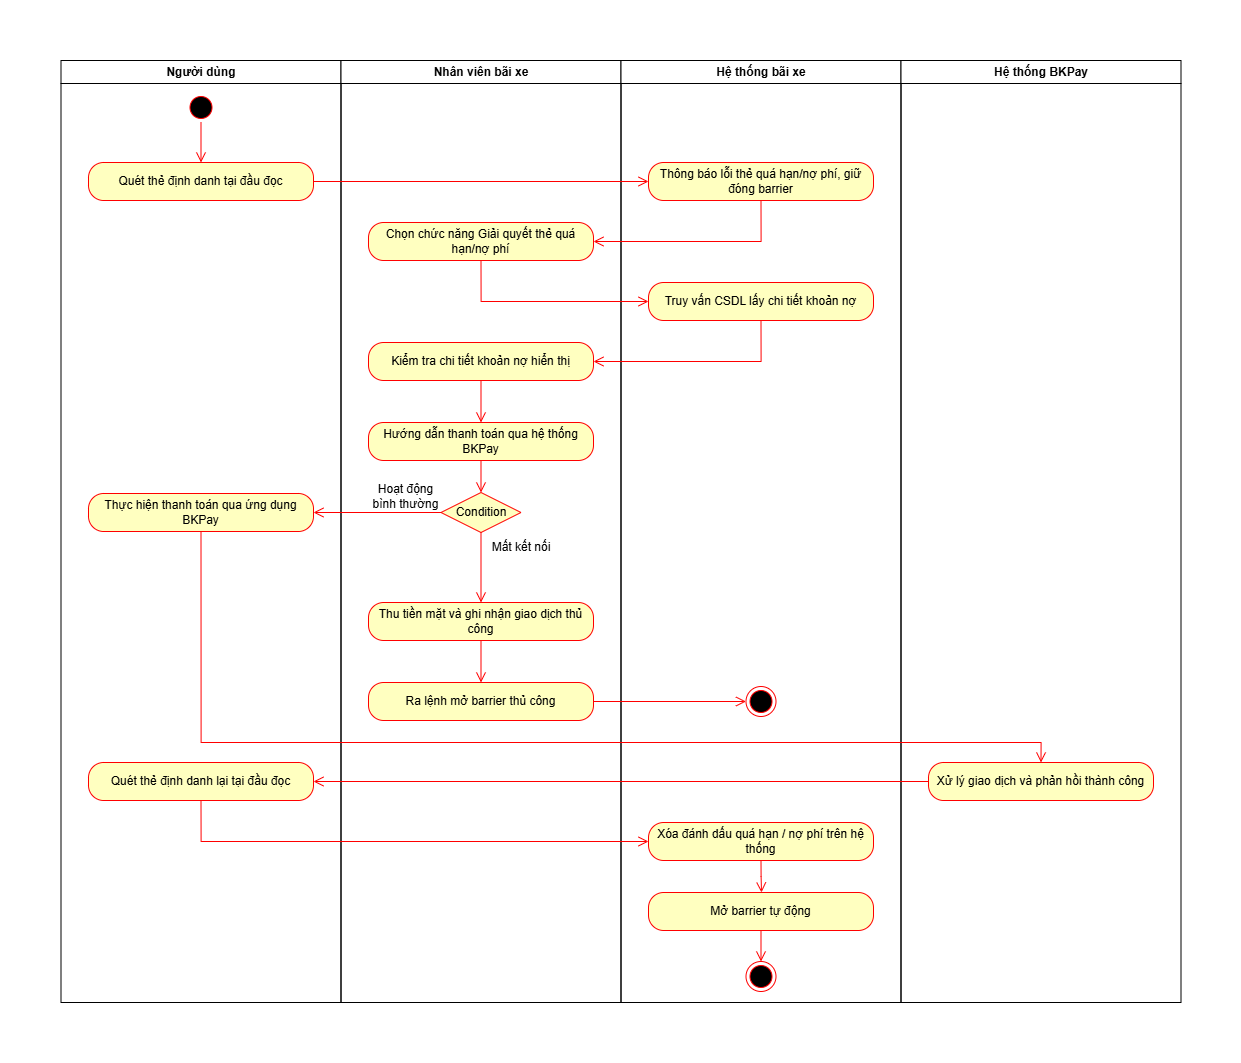
\includegraphics[width=0.9\textwidth, keepaspectratio]{../design/usecase-diagram/activity/overdue_card.png}
    \caption{Xử lý trường hợp đặc biệt - thẻ quá hạn}
\end{figure}

\subsubsection{Sơ đồ trình tự (Sequence Diagram)}
\begin{figure}[H]
    \centering
    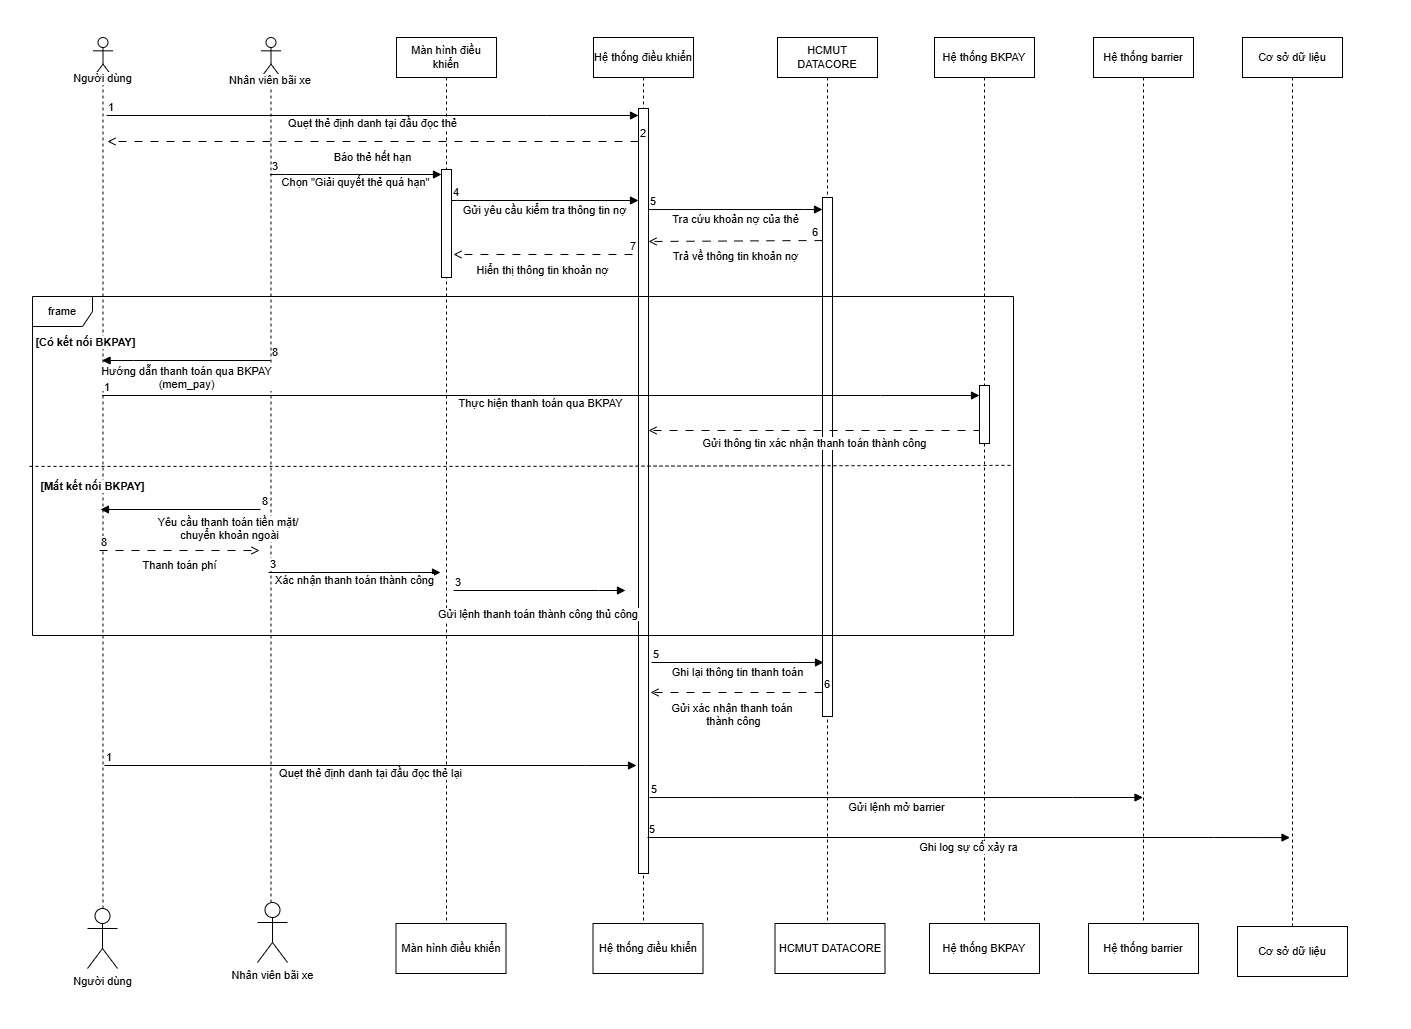
\includegraphics[angle=-90, origin=c, width=\textwidth, height=0.7\textheight, keepaspectratio]{../design/usecase-diagram/sequence/overdue_card.png}
    \caption{Xử lý trường hợp đặc biệt - thẻ quá hạn}
\end{figure}

% open_barrier_manual là spec_occ_6

\subsection{Xử lý trường hợp đặc biệt - mở rào thủ công}
\subsubsection{Sơ đồ hoạt động (Activity Diagram)}
\begin{figure}[H]
    \centering
    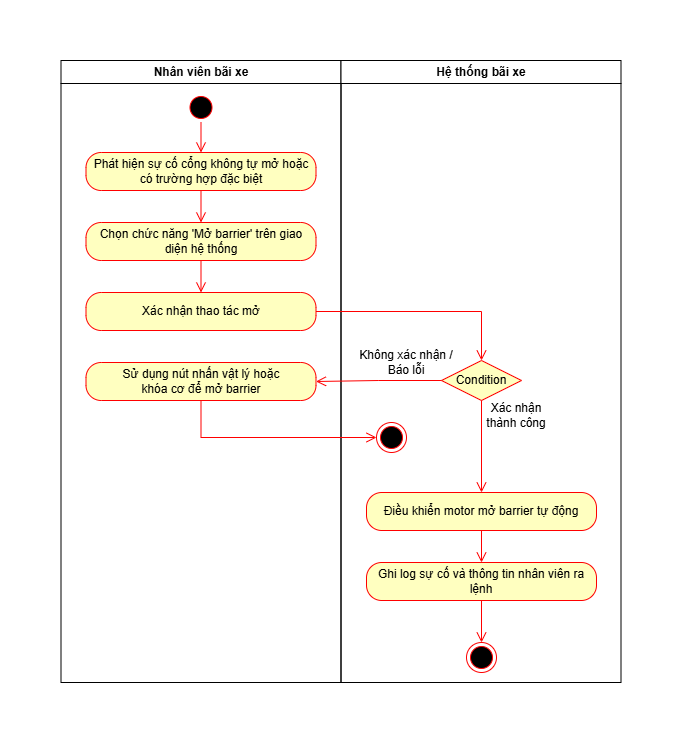
\includegraphics[width=0.9\textwidth, keepaspectratio]{../design/usecase-diagram/activity/open_barrier_manual.png}
    \caption{Xử lý trường hợp đặc biệt - mở rào thủ công}
\end{figure}

\subsubsection{Sơ đồ trình tự (Sequence Diagram)}
\begin{figure}[H]
    \centering
    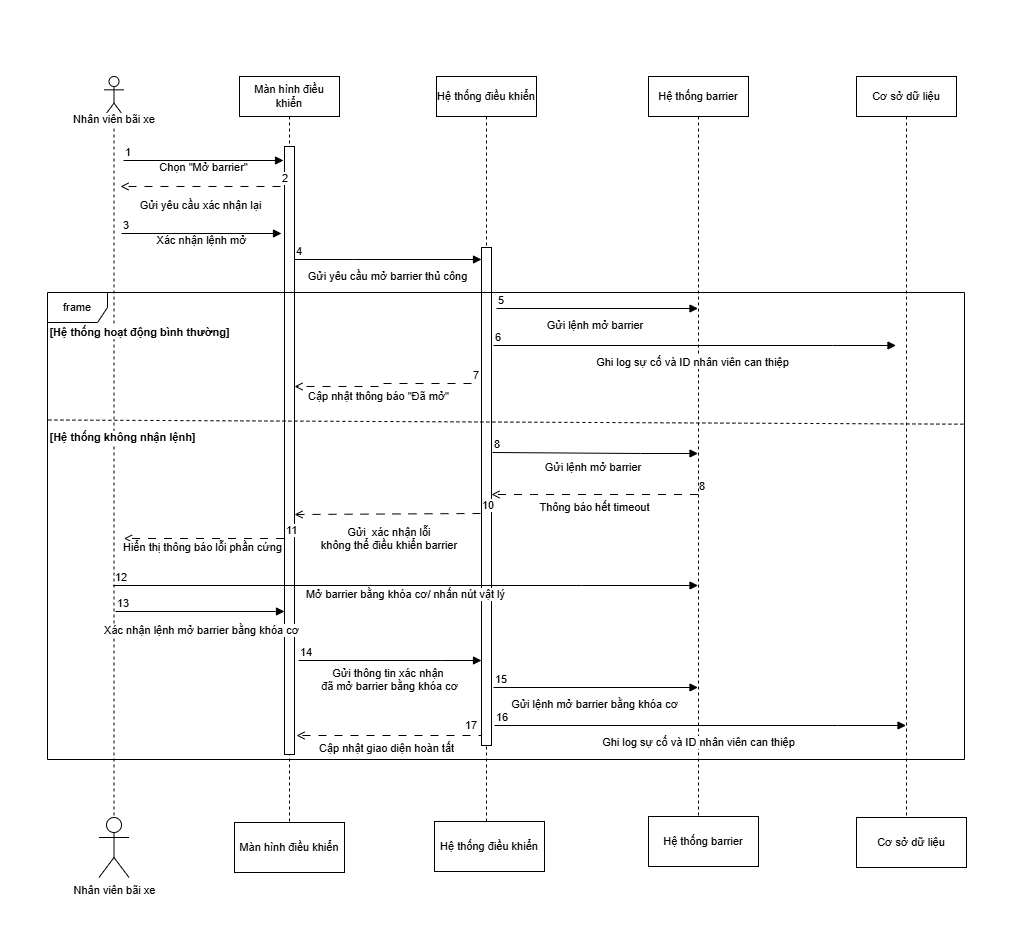
\includegraphics[angle=-90, origin=c, width=\textwidth, height=0.9\textheight, keepaspectratio]{../design/usecase-diagram/sequence/open_barrier_manual.png}
    \caption{Xử lý trường hợp đặc biệt - mở rào thủ công}
\end{figure}